\documentclass{manuscript}

% Additional packages not in manuscript.cls
\usepackage[T1]{fontenc}
\usepackage{booktabs}
\usepackage{amssymb}
\usepackage{array}
\usepackage{float}
\usepackage[section]{placeins}
\usepackage{needspace}
\usepackage{indentfirst}
\usepackage{tikz}
\usetikzlibrary{positioning,arrows,calc,shadows}
\usepackage{pgfplots}
\pgfplotsset{compat=1.18}

\graphicspath{{./images/}}

% PDF metadata
\hypersetup{pdfauthor={Ryan, K. R.}, pdftitle={The Geometric Siphon: Existence, Equilibrium, and Directional Properties of the Residual in Concentrated Liquidity Portfolios}}

\renewcommand{\thetheorem}{\arabic{theorem}}

\PassOptionsToPackage{hyphens}{url}
\Urlmuskip=0mu plus 1mu
\setlength{\emergencystretch}{3em}
\widowpenalty=10000
\clubpenalty=10000

\titleformat{\subsection}{\fontshape{it}\selectfont\bfseries}{\thesubsection.}{0.5em}{}
\titlespacing*{\subsection}{0pt}{10pt}{4pt}

\setlength{\intextsep}{8pt plus 2pt minus 2pt}
\setlength{\floatsep}{8pt plus 2pt minus 2pt}
\setlength{\textfloatsep}{10pt plus 2pt minus 2pt}

\AtBeginDocument{%
  \setlength{\abovedisplayskip}{18pt plus 3pt minus 2pt}%
  \setlength{\belowdisplayskip}{18pt plus 3pt minus 2pt}%
  \setlength{\abovedisplayshortskip}{14pt plus 2pt minus 1pt}%
  \setlength{\belowdisplayshortskip}{14pt plus 2pt minus 1pt}%
}


\newcolumntype{L}[1]{>{\raggedright\arraybackslash}p{#1}}
\renewcommand{\arraystretch}{1.2}
\AtBeginEnvironment{tabular}{\small}

\title{The Geometric Siphon:\\
Existence, Equilibrium, and Directional Properties of the Residual in Concentrated Liquidity Portfolios}
\author{K.\,R.~Ryan\thanks{K.\,R.~Ryan (\texttt{gancor@gancor.xyz}) is an independent researcher; ORCID 0009-0004-6295-7040.}}

\pagestyle{pagemain}

\pretitle{
  \centering \selectfont RESEARCH ARTICLE \par
  \fontsize{24pt}{28pt}\selectfont}

\begin{document}

\maketitle
\thispagestyle{pagefirst}

\begin{abstract}
This paper identifies and formalises the \emph{Geometric Siphon}, a previously undocumented mechanism arising from concentrated liquidity rebalancing geometry and made observable across positions by shared depositor balances. When autonomously rebalanced positions share a token balance, token ratio mismatches between old and new tick ranges route residual tokens through that shared balance, transferring capital between positions in independent pools. Six theorems characterise the mechanism. They establish a closed-form residual with an iff vanishing condition, convergence in expectation for same-pool positions sharing a contract balance, and geometric extinction without swap correction. On volatile/stablecoin pairs in V3 ordering, they also establish strict residual monotonicity in displacement together with USD-denominated directional and exit asymmetries. A graph-theoretic \emph{Connector Rule} relating per-pool flow to portfolio topology is stated as a conjecture. A 16-test Foundry suite verifies all six theorems against unmodified V3 contracts on Base mainnet. Empirically, a 1{,}380-event controlled dataset supports the existence claim, contains a complete USDC/ZARP extinction lifecycle, and includes an observed single-pool convergence episode. A separate 35{,}910-event production-scale dataset spanning five independent portfolios replicates the directional asymmetry in every portfolio, the exit asymmetry in four of five, and exhibits the predicted sign flip in the largest portfolio's reversed-ordering negative control.

\begin{keywords}
\item Concentrated liquidity.
\item Geometric residual.
\item Directional asymmetry.
\item Automated market maker.
\item Uniswap V3.
\end{keywords}
\end{abstract}

\let\item\olditem

\section{Introduction}\label{sec:introduction}

Concentrated liquidity, introduced in Uniswap V3,\cite{adams2021} requires active management. Every major CL automation platform (Gamma Strategies, Arrakis Finance, Beefy CLM) uses a \emph{vault-per-pool} architecture in which one vault manages one token pair and leftover tokens from rebalances are reinvested into the same position. Residuals stay in the pool that produced them and appear, if at all, as a small capital-efficiency loss difficult to separate from slippage.

Position Manager V6 (PMV6), a CL management contract on Base, accounts for residuals differently. Leftover tokens have no pool dimension and are held in \texttt{dustBalance[depositor][token]}, keyed by depositor and token only, so every position under one depositor draws from the same balance. That accounting choice opens a channel through which residuals from one pool can be consumed by positions in another. This paper characterises that channel and the residual that drives it.

On 2 March 2026, routine monitoring of one such PMV6 deployment revealed that a USDC/CHECK position had grown ${\sim}65\%$ while a USDC/ODOS position in the same depositor group had shrunk ${\sim}60\%$, although USDC was their only shared token. CHECK was consuming USDC residuals left behind by ODOS rebalances through the shared dust pool. The initial assumption was slippage; an on-chain decomposition of 92 rebalance transactions instead showed that the transfers were driven almost entirely by the geometric mismatch between consecutive tick ranges. I call this mechanism the \emph{Geometric Siphon}.

Cross-pool flow requires only that residuals be accessible through a shared balance across positions. This design choice is unusual in current production but not unique to PMV6, and any protocol that adopts it inherits the mechanism.

The discovery raises three questions: when does the residual vanish, what governs the long-run behaviour of positions exposed to it, and how does its USD-denominated value respond to price direction and exit type? Section~\ref{sec:theory} answers them in six theorems. A graph-theoretic \emph{Connector Rule}, tying per-pool flow direction to portfolio topology, is stated as a conjecture and supported empirically. A 16-test Foundry suite verifies all six theorems against unmodified V3 contracts on Base mainnet, six of them as live fork tests on Aerodrome Slipstream. A USDC/ZARP lifecycle ($\$942$ to $\$1.59$ in 14 zero-swap rebalances) illustrates Theorem~\ref{thm:extinction} at the average residual fraction.

Two operational datasets anchor the empirical results. A 1{,}380-event controlled phase spanning 39 positions over 7 days is consistent with the existence claim and contains both a single realisation of single-pool convergence and the full extinction lifecycle. A separate 35{,}910-event production-scale phase spanning 36 positions across five independent portfolios over 12 days replicates Theorems~\ref{thm:directional} and~\ref{thm:exit} within their volatile/stablecoin domain, with the reversed ordering subset as a built-in negative control.

Section~\ref{sec:related} places the paper in the V3 LP economics literature. The theoretical results and their main proof ideas follow next, with fuller derivations collected in Appendix~\ref{app:dr-derivation}. Section~\ref{sec:experimental} describes the Phase~1--3 design, and Section~\ref{sec:results} reports the results. Section~\ref{sec:foundry} summarises the Foundry verification, detailed in Appendix~\ref{app:foundry-detailed}. Section~\ref{sec:discussion} discusses the architectural precondition, the unit-of-account question, and the limitations. Section~\ref{sec:conclusion} concludes.

\section{Related work}\label{sec:related}

Concentrated liquidity in Uniswap V3\cite{adams2021} supplies the amount equations from which all six theorems derive.

Three lines of theoretical work model costs incurred by V3 LPs \emph{between} rebalances. Hasbrouck \emph{et al.}\cite{hasbrouck2025} model CL provision as a covered call sold at intrinsic rather than market value, so LPs forgo the option's time premium in exchange for fees; equilibrium liquidity provision decreases as that time premium rises. Cartea \emph{et al.}\cite{cartea2024} introduce \emph{predictable loss}, a closed-form measure of unhedgeable losses comprising convexity loss from informed trading and opportunity cost on locked capital, and analyse \emph{concentration risk}, the decrease in fee revenue when the marginal exchange rate exits the LP's range of liquidity. Milionis \emph{et al.}\cite{milionis2022b} introduce LVR (Loss-Versus-Rebalancing), the return gap between an AMM LP and a continuously rebalancing benchmark driven by arbitrage against stale AMM prices. Milionis \emph{et al.}\cite{milionis2024} extend the framework to fees and discrete block timing.

The geometric residual studied here is distinct from those loss mechanisms. It arises at the rebalance itself, is determined by the geometry of $R(s, s_a, s_b)$ rather than by price trajectory, exposure, or arbitrage, and is zero on same range rebalances regardless of price travel (Theorem~\ref{thm:residual}). The empirical decomposition in \S\ref{sec:decomposition} attributes over $97\%$ of observed Phase~1 flow to the residual rather than to swap-side friction. Theorems~\ref{thm:directional} and~\ref{thm:exit} identify USD-denominated asymmetries that are mechanistically separate from, but parallel in form to, the option-theoretic asymmetry of Hasbrouck \emph{et al.}\cite{hasbrouck2025} and the boundary-event behaviour analysed by Cartea \emph{et al.}\cite{cartea2024}.

Empirical work on V3 LPs has focused on per-position risk and return distributions. Heimbach \emph{et al.}\cite{heimbach2022} find wide cross-strategy variation that rewards active management. Willetts and Harrington\cite{willetts2026} measure arbitrage efficiency and rebalancing costs in dynamic-weight AMM pools on Ethereum and Base under LVR benchmarks, the closest published empirical context for per-rebalance cost analysis on Base L2. The empirical results below extend this line of work to a 35{,}910-event production-scale dataset focused specifically on rebalance-event dust flows.

Fan \emph{et al.}\cite{fan2023} formulate the LP's strategic problem as choosing tick ranges to maximise fees net of repositioning costs, treating each position in isolation. Theorems~\ref{thm:monotonicity}--\ref{thm:exit} characterise the asymmetries that any such strategy faces under directional price moves and at range exits.

Several alternative rebalancing architectures exist at the protocol level. Balancer\cite{martinelli2019} rebalances via its AMM invariant within a single pool; Set Protocol uses oracle-triggered swaps; Yearn deploys capital across strategist-managed strategies. All require a shared pool invariant, external price feeds, or manual intervention. Maverick Protocol's directional liquidity modes\cite{baxley2023} have bins follow price automatically; `Mode Both' is the closest analogue to siphon-driven repositioning, being continuous, automatic, and oracle-free, but operates within a single position. The Geometric Siphon arises from CL geometry alone and operates \emph{across} positions in different pools, requiring only a depositor-level shared dust balance.

Geometric residual flows between CL positions sharing depositor-level balances do not appear in the literature surveyed here. Nor do the directional and exit asymmetries of those residuals (Theorems~\ref{thm:directional}, \ref{thm:exit}), which follow from the same V3 amount equations.

A concurrent SSRN preprint by I.\,P.\cite{secondoperator2026} develops a graph-theoretic treatment of the same mechanism on a port of the present author's Position Manager to Uniswap V3. Its results are compatible with those here, including a residual-generation lemma equivalent to Theorem~\ref{thm:residual}, a circulation-path condition for cross-pool absorption (token degree $\geq 2$ in the portfolio graph), and a directional-convexity scaling for symmetric price displacements.

\clearpage
\section{Theoretical framework}\label{sec:theory}

Taken together, the results in this section proceed from existence to dynamics to asymmetry. Theorem~\ref{thm:residual} identifies when a rebalance does and does not generate a geometric residual, separating geometry-driven flow from slippage and motivating the decomposition tested in \S\ref{sec:decomposition}. Theorems~\ref{thm:convergence} and~\ref{thm:extinction} then characterise opposite dynamical regimes of the same mechanism, with Theorem~\ref{thm:convergence} giving expected same-pool convergence under shared balances and Theorem~\ref{thm:extinction} giving geometric extinction under repeated zero-swap rebalancing. Theorems~\ref{thm:monotonicity}--\ref{thm:exit} turn to displacement, direction, and exit type, showing how residual magnitude and retained USD value vary once a stablecoin num\'eraire is fixed. These results provide the formal link between the V3 amount equations and the production-scale directional patterns examined in \S\S\ref{sec:directional-empirical}--\ref{sec:exit-empirical}. Readers primarily interested in the empirical results may treat this section as a guide to the formal claims; full derivations are in Appendix~\ref{app:dr-derivation}.

\subsection{Concentrated-liquidity preliminaries}\label{sec:preliminaries}

The results below rely on the standard Uniswap V3 amount equations, the token ratio implied by a range at the current price, and the corresponding position value in token1 units.

\medskip
\noindent\emph{Token amounts in the position.}
\begin{equation}\label{eq:amounts}
x = L \left(\frac{1}{s} - \frac{1}{s_b}\right),
\qquad
y = L (s - s_a).
\end{equation}

\noindent\emph{Ratio of the two token amounts.}
\begin{equation}\label{eq:ratio}
R(s, s_a, s_b) = \frac{x}{y} = \frac{1/s - 1/s_b}{s - s_a}.
\end{equation}

\noindent\emph{Position value, in token1 units.}
\begin{equation}\label{eq:value}
V = x s^2 + y = L\,\phi(s, s_a, s_b),
\qquad
\phi(s, s_a, s_b) = 2s - \frac{s^2}{s_b} - s_a.
\end{equation}

\textbf{Notation.} The symbols used throughout the paper are summarised in Table~\ref{tab:notation} in Appendix~\ref{app:dr-derivation}.

\subsection{The geometric residual}\label{sec:residual}

A rebalance withdraws liquidity from $[s_a, s_b]$ and mints into $[s_a', s_b']$ at the same current price $s$. The withdrawn amounts are $x_w = L(1/s - 1/s_b)$ and $y_w = L(s - s_a)$. The new range requires the token ratio $R_{\text{new}} = R(s, s_a', s_b')$; if $R_{\text{old}} \neq R_{\text{new}}$, one withdrawn token is the binding constraint and the other is left in strict surplus.

The new liquidity is determined by the per-token minimum,
\begin{equation}\label{eq:lnew-min}
L_{\text{new}} = \min\!\left(\frac{x_w}{1/s - 1/s_b'}, \; \frac{y_w}{s - s_a'}\right),
\end{equation}
with the token1 term binding when $R_{\text{old}} \geq R_{\text{new}}$ (excess token0) and the token0 term binding when $R_{\text{old}} < R_{\text{new}}$ (excess token1).

Writing $\Delta R = V_{\text{new}} - V_{\text{old}}$ for the signed residual value of the rebalance in the isolated case, the residual fraction is $\Delta R/V = V_{\text{new}}/V_{\text{old}} - 1$, where $V_{\text{new}} = L_{\text{new}}\,\phi(s, s_a', s_b')$ and $V = V_{\text{old}}$ is the pre-rebalance value. In a shared balance setting, $D$ is the observed event-level dust flow and $D_{\text{pool}}$ the accumulated stock of contract dust available for absorption; $D/V$ can have either sign, depending on whether the mint absorbs surplus from $D_{\text{pool}}$ or contributes to it.

\begin{theorem}[Geometric residual]\label{thm:residual}
For a concentrated liquidity rebalance from range $[s_a, s_b]$ to $[s_a', s_b']$ at current sqrt price $s$, with $s$ contained in both ranges, consider the isolated case in which no shared balance tokens contribute to the mint. Let $\Delta R = V_{\text{new}} - V_{\text{old}}$ denote the signed residual value of the rebalance. Then
\[
\frac{\Delta R}{V} = 0 \;\iff\; R(s, s_a, s_b) = R(s, s_a', s_b').
\]
Equivalently, the rebalance has zero residual value if and only if the old and new ranges require the same token ratio at the current price. Range equality, $[s_a, s_b] = [s_a', s_b']$, is sufficient but not necessary.
\end{theorem}

\begin{proof}[Proof sketch]
($\Leftarrow$) If $R_{\text{old}} = R_{\text{new}}$, the withdrawn amounts $(x_w, y_w)$ already match the ratio required by the new range, so both tokens redeploy in full with no surplus. A direct substitution then gives $V_{\text{new}} = V_{\text{old}}$, hence $\Delta R/V = 0$. The substitution chain is given in Appendix~\ref{app:dr-derivation}.

($\Rightarrow$) If $R_{\text{old}} \neq R_{\text{new}}$, by~\eqref{eq:lnew-min} exactly one token binds the new liquidity and the other remains in strict surplus, exiting the mint as dust with strictly positive token value $|\Delta R|$. By token value conservation, $V_{\text{new}} = V_{\text{old}} - |\Delta R| < V_{\text{old}}$, so $\Delta R = V_{\text{new}} - V_{\text{old}} < 0$ and in particular $\Delta R/V \neq 0$. This establishes the reverse implication by contrapositive.
\end{proof}

\subsection{Two-mechanism structure}\label{sec:two-mechanism}

Theorem~\ref{thm:residual} partitions rebalances into ratio-changing events ($\Delta R \neq 0$) and ratio-preserving events ($\Delta R = 0$). In Phase~2, only about 5\% of events are ratio-changing; the other 95\% are ratio-preserving (\S\ref{sec:two-mechanism-split}). Same-range events nonetheless produce non-zero mean $|D|$, which only a contract-level dust pool can explain.

\textbf{Stage~1: Geometric creation.} Range-change rebalances produce geometric residuals via~\eqref{eq:lnew-min}. PMV6's internal swap absorbs about 94\% of the ratio mismatch; the remainder enters the shared dust pool as unmatched tokens. Without range changes, the pool is no longer replenished and drains towards zero.

\textbf{Stage~2: Dust-pool redistribution.} Same-range rebalances draw from accumulated contract dust. The CL mint function uses all available tokens,
\begin{equation}\label{eq:mint}
L_{\text{new}} = \min\!\left(\frac{x_w + x_{\text{dust}}}{1/s - 1/s_b'}, \; \frac{y_w + y_{\text{dust}}}{s - s_a'}\right),
\end{equation}
so excess pool dust on the non-binding side is absorbed ($D > 0$), while a slight imbalance in the withdrawn amounts can leave residual dust ($D < 0$).

The siphon requires all three components. Removing any one shuts the mechanism off in a different way.

\begin{table}[H]
\centering
\caption{Necessary components of the siphon mechanism.}
\label{tab:siphon-components}
\renewcommand{\arraystretch}{1.05}
\begin{tabular}{@{}lll@{}}
\toprule
Remove \dots & Effect & Siphon? \\
\midrule
Range changes (Stage~1)     & No residual is created                  & Stops; pool drains to zero \\
Same-range events (Stage~2) & Dust accumulates but is never absorbed & Stops; tokens remain stranded \\
Shared balances             & Each position's dust remains isolated  & Stops; no transfer medium \\
\bottomrule
\end{tabular}
\end{table}

In steady state, the two flows balance. On the same range branch, the sign of $D$ is governed by $V/L_p$; the empirical crossover is mapped in \S\ref{sec:vl-sweep}.

\subsection{Equilibrium}\label{sec:equilibrium}

Within a single pool, residuals donated by one rebalance become dust available for later rebalances to absorb. Larger positions donate proportionally, while smaller positions receive a larger proportional benefit from any given dust absorption. Same-pool values therefore converge in expectation.

\begin{theorem}[Single-pool convergence]\label{thm:convergence}
$N$ positions in the same pool and range, sharing a contract balance, converge in expectation to equal value under repeated rebalancing with uniform per-position rebalance probability.
\end{theorem}

\begin{proof}
Geometric donation is proportional to liquidity, so the per-event donation $|\Delta R_i|$ scales with $V_i$, and the proportional donation rate is approximately position-size-independent on the same range branch (\S\ref{sec:vl-sweep}). By contrast, the mint constraint~\eqref{eq:mint} consumes the available dust pool in absolute terms, so the proportional gain from absorption is inversely proportional to position size.

With per-position rebalance probability $\pi = 1/N$,
\begin{equation}\label{eq:growth}
\mathbb{E}\!\left[\frac{\dot{V}_i}{V_i}\right]
=
\underbrace{\frac{\pi D_{\text{pool}}}{V_i}}_{\text{absorption}\,\propto\,1/V_i}
-
\underbrace{c}_{\text{donation (constant)}}.
\end{equation}
The first term is strictly decreasing in $V_i$, while the second is constant, so smaller positions grow faster in proportional terms. Equilibrium, defined by $\dot{V}_i/V_i = \dot{V}_j/V_j$, therefore requires $V_i = V_j$. In the regime where the linearisation holds, the resulting gradient contracts towards that fixed point.
\end{proof}

\begin{corollary}[Exponential convergence rate]\label{cor:convergence-rate}
Under the assumptions of Theorem~\ref{thm:convergence} and the additional assumption that swap routing preserves total value (so $\sum_i V_i + D_{\text{pool}}$ is constant in expectation), the differential deviations between positions decay exponentially at rate $c$:
\[
\bigl|\mathbb{E}[V_i(t) - V_j(t)]\bigr|
\leq
|V_i(0) - V_j(0)|\,e^{-ct}
\qquad \forall\, i,j.
\]
The decay timescale is $\tau = 1/c$, independent of $N$. Proof in Appendix~\ref{app:dr-derivation}.
\end{corollary}

\noindent Across pools with total liquidities $L_{p,k}$, the same argument extends to
\begin{equation}\label{eq:multipool}
\frac{V_i}{L_{p,k(i)}}
=
\frac{V_j}{L_{p,k(j)}}
\qquad \forall\, i,j,
\end{equation}
so positions in deeper pools settle at larger values. Hub-spoke topologies therefore reach equilibrium with the deep hub sustaining a larger position and the shallower spokes sustaining smaller ones (\S\ref{sec:predictive}).

\subsection{The Connector Rule (conjectural)}\label{sec:connector}

With shared balances across multiple pools, the identity of the per-pool driver token follows a simple empirical regularity. For a portfolio with positions in pools $\{P_k\}$, define the connectivity of token $T$ by
\[
\mathrm{conn}(T) = \bigl|\{k : T \in P_k\}\bigr|.
\]
The empirical evidence is reported in \S\ref{sec:predictive}.

\begin{conjecture}[Connector Rule]
In pool $P_k = (T_a, T_b)$, the siphon driver is the token with higher connectivity,
\[
\arg\max_{T \in \{T_a, T_b\}} \mathrm{conn}(T),
\]
when the maximiser is unique; ties are not addressed here.
\end{conjecture}

A cross-group check on the WETH/USDC pool across three depositor groups is consistent with this rule (\S\ref{sec:predictive}). The driver token is the side with higher connectivity in the rest of the portfolio: WETH in a WETH-hub group and USDC in a USDC-hub group.

When the connector token moves, every pool containing it experiences a correlated geometric mismatch on that side, whereas the non-connector token follows pool-specific dynamics. Correlated mismatches in the connector leg can therefore generate systematic net flows, while mismatches in peripheral tokens tend to average out.

\subsection{Zero-swap extinction}\label{sec:extinction}

In pools with swap routing, PMV6's internal swap absorbs about 94\% of $\Delta R$ at each rebalance, leaving only about 6\% as net dust. This damping keeps positions inside the convergence basin of Theorem~\ref{thm:convergence}. When swap routing is unavailable ($S = 0$ on every event, as in a stablecoin pair with no DEX path), that damping is absent and the full residual leaks on each rebalance. The USDC/ZARP lifecycle (\S\ref{sec:zarp}) provides the empirical example.

\begin{theorem}[Zero-swap extinction]\label{thm:extinction}
Let $P$ be a CL position with value $V_0 > 0$. If the current price exits the position's range and a rebalance is performed with $S = 0$ (no swap), minting into a new range containing the current price, then:
\begin{enumerate}
\item $V_1 < V_0$.

\item The residual fraction
\[
\alpha = \frac{V_0 - V_1}{V_0} > 0
\]
is non-decreasing in $|\delta|/w$ and saturates at $1$.

\item After $K$ consecutive zero-swap rebalances,
\[
V_K = V_0 \prod_{k=1}^{K} (1 - \alpha_k),
\]
with bounds
\[
V_K \leq V_0(1 - \bar\alpha_K)^K,
\qquad
V_K \leq V_0(1 - \alpha_{\min})^K.
\]

\item The position reaches any $\varepsilon > 0$ in at most
\[
K^* = \left\lceil \frac{\ln(V_0/\varepsilon)}{\ln(1/(1 - \bar\alpha))} \right\rceil,
\qquad
K^*_{\text{loose}} = \left\lceil \frac{\ln(V_0/\varepsilon)}{\ln(1/(1 - \alpha_{\min}))} \right\rceil.
\]
\end{enumerate}
\end{theorem}

\begin{proof}[Proof sketch]
\emph{Part (i).} At an above-range exit, $x_w = 0$ and $y_w = L(s_b - s_a)$, so the withdrawn position is entirely token1. The new range is centred on the current price and therefore requires both tokens. In the isolated case, token0 is absent, so the mint constraint~\eqref{eq:mint} gives $L_{\text{new}} = 0$, hence $\alpha = 1$. With a finite shared dust pool, some missing token0 may be supplied, but not enough to eliminate the loss entirely, so $0 < \alpha \leq 1$ and $V_1 < V_0$. The below-range case is symmetric at the level of residual fraction; the difference in USD value between the two sides is treated separately in Theorem~\ref{thm:exit}.

\emph{Part (ii).} The premise implies $|\delta| \geq w/2$. As $|\delta|$ increases further beyond the boundary, the withdrawn amount of the binding token remains zero, while the recentred range continues to require that token for redeployment. The unrecoverable fraction therefore cannot decrease, so $\alpha$ is non-decreasing in $|\delta|/w$ and saturates at $1$. At the boundary $|\delta| = w/2$, this matches Theorem~\ref{thm:monotonicity} continuously, since $|\Delta R(\pm w/2)|$ is the full single-sided balance on each branch.

\emph{Parts (iii)--(iv).} Repeated application of Part~(i) gives
\[
V_K = V_0 \prod_{k=1}^{K} (1 - \alpha_k).
\]
Applying AM--GM to the positive terms $\{1 - \alpha_k\}$ yields the stated bounds, and solving $V_0(1 - \bar\alpha)^K \leq \varepsilon$ for $K$ gives the extinction time. The full derivation is in Appendix~\ref{app:dr-derivation}.
\end{proof}

\noindent Under sustained $S = 0$ with stable or declining pool liquidity $L_p$, the sequence $V_0, V_1, \ldots$ is monotonically decreasing. The trajectory cannot recover endogenously. As $V$ shrinks while $L_p$ is constant or declining, $V/L_p$ is non-increasing, so the position remains in the donation regime.

\begin{corollary}[Irreversibility of zero-swap extinction]\label{cor:irreversibility}
Under the assumptions of Theorem~\ref{thm:extinction}, the position cannot return to net absorption without an exogenous change in pool liquidity. Specifically, recovery requires $L_p$ to increase enough that $V/L_p$ falls below the absorption crossover identified empirically in \S\ref{sec:predictive}.
\end{corollary}

\noindent The crossover separates the convergence regime of Theorem~\ref{thm:convergence}, in which same-pool positions absorb in expectation, from the extinction regime of Theorem~\ref{thm:extinction}, in which a position with $S = 0$ donates on every rebalance. The intermediate case $0 < S_{\text{eff}} < 1$, where $S_{\text{eff}}$ is the fraction of $\Delta R$ recovered by the swap, is not characterised here. In the empirical record, every observed recovery on the USDC/ZARP trajectory (\S\ref{sec:zarp}) coincided with a substantial increase in $L_p$, consistent with this corollary.

\subsection{Residual monotonicity}\label{sec:monotonicity}

The equal-width rebalance recentred on the current price is the canonical policy of automated CL engines, including the one in \S\ref{sec:infrastructure}. Theorem~\ref{thm:monotonicity} characterises how the residual changes as the current price moves away from the midpoint of the original range.

\begin{theorem}[Residual monotonicity]\label{thm:monotonicity}
For a CL position in range $[s_a, s_b]$ rebalanced to a new range of equal width centred on the current sqrt price $s$, where $s$ has been displaced by $\delta$ from the midpoint $\bar{s} = (s_a + s_b)/2$, the absolute geometric residual $|\Delta R|$ is strictly increasing in $|\delta|$ on $(0, w/2]$, with $\Delta R(0) = 0$ and $\Delta R(w/2) = L \cdot w$. The boundary magnitude on the downward branch is smaller by a factor of $\bar{s}/s_b$ (Theorem~\ref{thm:directional}).
\end{theorem}

\begin{proof}[Proof sketch]
Let $w = s_b - s_a$, $\bar{s} = (s_a + s_b)/2$, and $s = \bar{s} + \delta$. At $\delta = 0$, the old and new ranges require the same token ratio, so $\Delta R(0) = 0$ by Theorem~\ref{thm:residual}. For $\delta > 0$, the old position becomes increasingly token1-heavy, while the recentred range requires relatively more token0. Token0 therefore binds, and the residual appears as surplus token1:
\begin{equation}\label{eq:dr-closed-form}
\Delta R(\delta) = L(s - s_a) - L\!\left(\frac{1/s - 1/s_b}{1/s - 1/(s + w/2)}\right)(w/2).
\end{equation}
Appendix~\ref{app:dr-derivation} simplifies~\eqref{eq:dr-closed-form} and shows that its derivative is strictly positive on $(0, w/2]$, with $\Delta R(0) = 0$ and $\Delta R(w/2) = L \cdot w$. The downward branch is also strictly monotone in $|\delta|$, with boundary magnitude smaller by a factor of $\bar{s}/s_b$ (Theorem~\ref{thm:directional}), so $|\Delta R|$ is strictly increasing in $|\delta|$ on $(0, w/2]$.
\end{proof}

\subsection{Directional asymmetry}\label{sec:directional}

Beyond the range-geometric asymmetry of Theorem~\ref{thm:monotonicity}, the retained USD value at $+\delta$ strictly exceeds that at $-\delta$ once a stablecoin num\'eraire is fixed. Throughout this subsection, $V(s \pm \delta)$ denotes $L\,\phi(s \pm \delta, s_a, s_b)$, the position value evaluated at the displaced sqrt price with the range $[s_a, s_b]$ held fixed.

\begin{theorem}[Directional asymmetry]\label{thm:directional}
For a CL position in pool $(T_0, T_1)$ with $T_0$ the volatile asset and $T_1$ a stablecoin, the up-move position $V(s+\delta)$ retains strictly more USD value than the down-move position $V(s-\delta)$ at every $\delta > 0$ for which both $s \pm \delta$ remain in range.
\end{theorem}

\begin{proof}
With $V = L\,\phi(s, s_a, s_b)$ and $\phi(s, s_a, s_b) = 2s - s^2/s_b - s_a$, direct expansion gives
\begin{equation}\label{eq:directional-identity}
V(s + \delta) - V(s - \delta) = 4 L \delta \left(1 - \frac{s}{s_b}\right).
\end{equation}
For any $s$ in the interior of $[s_a, s_b]$, the factor $(1 - s/s_b)$ is strictly positive, so $V(s+\delta) > V(s-\delta)$ at every admissible $\delta > 0$.
\end{proof}

Substituting $\delta = \Delta P/(2s)$ into~\eqref{eq:directional-identity} yields a leading-order price-space scaling of the asymmetry that vanishes continuously as $s \to s_b$; the explicit formula is given in Appendix~\ref{app:dr-derivation} (Cor.~\ref{cor:directional-scaling}). Combined with the range-geometric asymmetry of Theorem~\ref{thm:monotonicity}, USD-denominated residual magnitudes on volatile/stablecoin pairs are therefore asymmetric in $\delta$. The asymmetry is num\'eraire-dependent: in token0 units the inequality reverses, so the apparent USD bias reflects the standard token ordering rather than a direction-dependent geometric residual.

\subsection{Exit asymmetry}\label{sec:exit}

Past the range boundary, the position is single-sided. In V3 ordering for volatile/stablecoin pairs, above-exits hold only the stablecoin and retain full USD value, while below-exits hold only the depreciated volatile token.

\begin{theorem}[Exit asymmetry]\label{thm:exit}
For a CL position in pool $(T_0, T_1)$ with $T_0$ the volatile asset and $T_1$ a stablecoin, a below-range exit retains strictly less USD value than an above-range exit at any sqrt-price displacement $d > 0$ past the corresponding boundary.
\end{theorem}

\begin{proof}[Proof sketch]
Let $d > 0$ denote the sqrt-price displacement past the relevant boundary, with $d < s_a$ in the below-exit case so that $s_a - d > 0$. At an above-exit ($s' = s_b + d$), the position holds only token1 with
\[
V_{\text{above}} = L(s_b - s_a),
\]
which equals USD in stablecoin units and is constant in $d$. At a below-exit ($s' = s_a - d$), the position holds only token0 with quantity
\[
x_{\text{below}} = L\left(\frac{1}{s_a} - \frac{1}{s_b}\right),
\]
and at the prevailing market price $s'^2 = (s_a - d)^2$,
\begin{equation}\label{eq:vbelow}
V_{\text{below}}(d) = L\left(\frac{1}{s_a} - \frac{1}{s_b}\right)(s_a - d)^2.
\end{equation}
This is strictly decreasing in $d$ on $(0, s_a)$. Hence $V_{\text{below}}/V_{\text{above}}$ is strictly decreasing in $d$, and the below-exit retains strictly less USD value at every $d > 0$.
\end{proof}

\begin{corollary}[Closed-form exit value-retention ratio]\label{cor:exit-ratio}
Under the conditions of Theorem~\ref{thm:exit},
\[
\frac{V_{\text{below}}(d)}{V_{\text{above}}}
=
\frac{(s_a - d)^2}{s_a s_b}
=
\frac{P'}{\sqrt{P_a P_b}},
\]
with $P' = (s_a - d)^2$, $P_a = s_a^2$, and $P_b = s_b^2$. The ratio is strictly decreasing in $d$, from $\sqrt{P_a/P_b} < 1$ as $d \to 0^+$ to $0$ as $d \to s_a^-$. Dividing $V_{\text{below}}$ by $V_{\text{above}}$ from~\eqref{eq:vbelow} and using $s_a s_b = \sqrt{P_a P_b}$ yields the closed form.
\end{corollary}

\section{Experimental design}\label{sec:experimental}

The empirical work spans three phases on Aerodrome (Base): a 41.9-hour mechanism-discovery phase on PMV6, a controlled formalisation window on PMV7, and a 12-day production-scale phase on PMV8--PMV9. Phase~1 was terminated early by a contract exploit on 5~March that corrupted depositor state; the production-scale rebalances that continued from 6~March under non-diffusion logging during the PMV7 redeploy are excluded from Phase~3. The production-scale checks of \S\S\ref{sec:directional-empirical}--\ref{sec:exit-empirical} therefore use PMV8--PMV9 only.

\begin{table}[H]
\centering
\caption{The three experimental phases.}
\label{tab:phases-overview}
\begin{tabular}{@{}lL{3.5cm}L{3.5cm}L{3.5cm}@{}}
\toprule
 & Phase 1 & Phase 2 & Phase 3 \\
\midrule
Role      & Mechanism discovery & Formalisation, controlled verification & Production-scale replication \\
Period    & 3--5 Mar 2026 (41.9 h) & 7--12 Mar 2026 & 13--24 Mar 2026 \\
Contract  & PMV6 & PMV7 (controlled subset) & PMV8--PMV9 \\
Positions & 22, in 5 groups & 17, in 5 groups & 36, in 5 portfolios \\
Events    & 738 diffusion, 1{,}192 rebalances & 642 diffusion & 35{,}910 rebalances \\
Design    & Controlled & Controlled & Operational \\
\bottomrule
\end{tabular}
\end{table}

\subsection{Infrastructure}\label{sec:infrastructure}

All three phases used the same adaptive rebalancing engine. The engine monitors pool swap events via WebSocket, computes rolling volatility $\sigma$ over 1h, 4h, and 24h windows, and triggers a rebalance whenever the current tick exits the position's range. The new range is centred on the current tick, with width $w = C \cdot \sigma \cdot \sqrt{t}$, where $C \in \{2, 3, 4\}$ in the datasets reported here. Each rebalance is executed as a single atomic call: withdraw $\to$ optional swap $\to$ mint $\to$ stake. All rebalances are autonomous, with no human intervention between deployment and data collection.

\subsection{Phase 1: Mechanism discovery}\label{sec:phase1}

\begin{table}[H]
\centering
\caption{Phase 1 group design.}
\label{tab:phase1-groups}
\begin{tabular}{@{}clL{8.5cm}l@{}}
\toprule
Group & Positions & Design & Key variable \\
\midrule
A & 3 & Similar $V/L_p$, different volatility & $\sigma$ isolation \\
B & 7 & Pre-existing mix of CL1/CL10/CL100, 5 shared tokens & Diversity \\
C & 2 & Same pool (EURC/USDC CL1), isolated address & Same-pool control \\
D & 5 & \$500 each, identical policy, $30\times$ TVL spread & Pool TVL \\
E & 5 & Matched TVL (${\sim}\$190$--$323$K), $183\times$ emission spread & Emission rate \\
\bottomrule
\end{tabular}
\end{table}

\subsection{Phase 2: Formalisation and verification}\label{sec:phase2}

\begin{table}[H]
\centering
\caption{Phase 2 group design.}
\label{tab:phase2-groups}
\setlength{\tabcolsep}{4pt}
\begin{tabular}{@{}clL{9.2cm}l@{}}
\toprule
Group & Positions & Design & Key variable \\
\midrule
A & 3 & WETH/USDC hub + CLAWD/USDC + WETH/AERO & Topology \\
B & 4 & WETH/USDC hub + WETH/VVV + WETH/AERO + USDC/CHECK & Cross-pool flow \\
C & 5 & EURC/USDC + four exotic FX pairs (all USDC-paired) & $\sigma \approx 0$ isolation \\
D & 2 & WETH/USDC + WETH/EURC & Connector test \\
E & 3 & Same pool (KellyClaude/USDC), deployed at 1{:}3{:}9 & Single-pool equilibrium \\
\bottomrule
\end{tabular}
\end{table}

\noindent\textbf{Key Phase 2 design features.}

\textbf{Hub-spoke topology.} WETH/USDC CL50 served as the central hub, with each spoke sharing either WETH or USDC.

\textbf{$V/L_p$ sweep.} Three positions were deployed in the same pool at a $1{:}3{:}9$ size ratio, isolating position size as the only varying factor.

\textbf{Fiat-FX weekend experiment.} Five stablecoin FX pairs were deployed on a Sunday, when markets were closed, under $\sigma \approx 0$ conditions that isolate the $V/L_p$ effect from volatility.

\subsection{Phase 3: Production-scale directional check}\label{sec:phase3}

Unlike Phases~1--2, Phase~3 was operational rather than controlled. The five depositor groups arose from the operator's deployment topology rather than experimental design, and \S\S\ref{sec:directional-empirical}--\ref{sec:exit-empirical} use them as five independent per-portfolio replications. Phase~3 provides the production-scale replications of Theorems~\ref{thm:directional} and~\ref{thm:exit}; the smaller controlled designs of Phases~1--2 provide the case-study evidence for Theorems~\ref{thm:residual}--\ref{thm:extinction}.

\subsection{Hypotheses (Phases 1--2)}\label{sec:hypotheses}

\begin{table}[H]
\centering
\caption{Hypotheses for the controlled phases.}
\label{tab:hypotheses}
\begin{tabular}{@{}lL{6.4cm}lL{4cm}@{}}
\toprule
ID & Hypothesis & Source & Result \\
\midrule
H1 & Flow is geometric; same range $\Delta R = 0$ & Theory (Thm~\ref{thm:residual}) & Yes, $\rho = 0.976$; 611/611 \\
H2 & $V/L_p$ and $\sigma$ are complementary predictors & Phase~1 & Yes, Simpson's paradox confirmed \\
H3 & Same-pool positions converge & Theory (Thm~\ref{thm:convergence}) & Yes, $1{:}3{:}9 \to 1.37{:}1{:}1.20$ \\
H4 & Multi-pool positions settle at equal $V/L_p$ & Theory~\eqref{eq:multipool} & Yes, hub-spoke stable \\
H5 & The siphon driver is the connector token & Theory (\S\ref{sec:connector}) & Yes, 10-pool cross-group \\
H6 & $\sigma = 0$ isolates $V/L_p$ as the dominant predictor & Phase~2 design & Yes, fiat-FX consistent \\
\bottomrule
\end{tabular}
\end{table}

\noindent Phase~3 is not part of this hypothesis-testing framework; see \S\S\ref{sec:directional-empirical}--\ref{sec:exit-empirical} for its production-scale role.

\section{Results}\label{sec:results}

\subsection{Core decomposition: \texorpdfstring{$D = \Delta R - S$}{D = Delta R - S}}\label{sec:decomposition}

Swap event logs from 92 on-chain Phase~1 rebalance transactions were decoded to recover realised swap amounts.

\begin{table}[H]
\centering
\caption{Core decomposition of observed dust flow.}
\label{tab:decomposition}
\begin{tabular}{@{}lrr@{}}
\toprule
Metric & Value & $N$ \\
\midrule
Spearman $\rho(\Delta R, D)$     & \textbf{0.976} & 72 \\
Spearman $\rho(|\Delta R|, |D|)$ & \textbf{0.947} & 72 \\
Events with swap                 & 72             & --- \\
Events without swap              & 20             & --- \\
Mean slippage $S$                & \$1.49         & 72 \\
Median swap price impact         & \textbf{0.35\%} & 72 \\
\bottomrule
\end{tabular}
\end{table}

Among the 72 transactions involving a swap, the residual is strongly rank-correlated with observed flow: $\rho(\Delta R, D) = 0.976$ and $\rho(|\Delta R|, |D|) = 0.947$. Mean slippage is \$1.49, with median price impact of $0.35\%$.

Across the full Phase~1 dataset of 738 events, 536 events ($73\%$) involved on-chain swaps and accounted for $97\%$ of gross dollar flow. Swap costs therefore act as a small offset to the residual signal across the dataset.

\subsection{Predictive analysis and Simpson's paradox}\label{sec:predictive}

\subsubsection{Aggregate versus stratified correlations}

Pooling all 545 events with $|D| > \$0.50$ gives $\rho = 0.329$ for $V/L_p$ and $\rho = -0.367$ for $\sigma$, which in aggregate suggests that higher volatility is associated with smaller flows. Stratifying by portfolio group reverses that result, producing a Simpson's paradox. Table~\ref{tab:stratified-correlations} reports the per-group Spearman correlations of $|D|$ against $V/L_p$ and $\sigma_{1h}$.

\begin{table}[H]
\centering
\vspace{-10pt}\caption{Stratified $|D|$ correlations.}
\label{tab:stratified-correlations}
\begin{tabular}{@{}lrrr@{}}
\toprule
Group & $N$ & $V/L_p \to |D|$ & $\sigma_{1h} \to |D|$ \\
\midrule
A & 75  & 0.054           & \textbf{0.575} \\
B & 114 & \textbf{0.562}  & $-0.362$ \\
C & 55  & 0.210           & $-0.082$ \\
D & 178 & 0.171           & $0.086$ \\
E & 123 & \textbf{0.370}  & $-0.321$ \\
\bottomrule
\end{tabular}
\end{table}

$V/L_p$ and $\sigma$ are informative in different regimes. Each becomes more predictive when the other shows little cross-position variation. Group~B mixes CL1, CL10, and CL100 positions, producing an approximately $25\times$ spread in $V/L_p$; accordingly, $V/L_p$ explains much of the observed variation there. Group~A, by contrast, has near-identical $V/L_p$, so $\sigma$ carries more of the explanatory signal.

The aggregate sign reversal is driven by pool size. High-$\sigma$ pools also tend to be thin, so they generate smaller absolute dollar flows even when their relative mismatches are larger.

\subsubsection{Non-linear $V/L_p$ transfer function}

The relationship between $V/L_p$ and $D/V$ is non-monotonic. Bucketed Phase~2 event data through 9~March ($N = 606$; Appendix~\ref{app:empirical}, Table~\ref{tab:vl-buckets}) show that absorption peaks around $V/L_p \approx 0.05$--$0.10$, crosses zero near $(V/L_p)^{*} \approx 0.13$, and then shifts into increasingly strong donation above that point (Fig.~\ref{fig:vl-transfer}). Each observation is a single rebalance event for one position. The contract's depositor-keyed dust balance prevents flow between portfolios, so the pattern reflects within-portfolio dynamics only.

Because $73\%$ of events lie at $V/L_p < 0.01$, a linear regression is misleading here ($r \approx -0.1$). The bucketed pattern is more informative. Volatility increases magnitude, with Pearson $r = 0.26$ between $\sigma_{1h}$ and $|D/V|$ for $N = 536$, but it does not determine direction.

\vspace{8pt}
\begin{figure}[H]
\centering
\definecolor{cryptoblue}{HTML}{2C5F8D}
\definecolor{fiatorange}{HTML}{C0392B}
\definecolor{absorbtint}{HTML}{E8F4EC}
\definecolor{donatetint}{HTML}{FBEEEC}
\begin{tikzpicture}
\begin{axis}[
  width=0.9\linewidth, height=9cm,
  xlabel={$V/L_p$ (log scale)},
  ylabel={Mean $D/V$},
  xmode=log,
  log basis x=10,
  xmin=0.004, xmax=1.6,
  ymin=-0.42, ymax=0.32,
  xtick={0.01, 0.1, 1},
  xticklabels={0.01, 0.1, 1},
  ytick={-0.4, -0.3, -0.2, -0.1, 0, 0.1, 0.2, 0.3},
  scaled y ticks=false,
  yticklabel style={/pgf/number format/.cd, fixed, fixed zerofill, precision=1},
  minor x tick num=9,
  minor y tick num=4,
  axis x line=bottom, axis y line=left,
  axis line style={black!55, line width=0.4pt, -},
  tick style={black!55, line width=0.4pt},
  minor tick style={black!30, line width=0.3pt},
  every axis label/.style={font=\small},
  every tick label/.style={font=\footnotesize},
  clip=false,
]

% Background regime tinting (absorption | donation), drawn first to sit behind
\path[fill=absorbtint] (axis cs:0.004, -0.42) rectangle (axis cs:0.13, 0.32);
\path[fill=donatetint] (axis cs:0.13, -0.42) rectangle (axis cs:1.6, 0.32);

% Zero line and crossover guide
\draw[dashed, draw=black!40, line width=0.5pt]
  (axis cs:0.004, 0) -- (axis cs:1.6, 0);
\draw[densely dotted, draw=black!50, line width=0.6pt]
  (axis cs:0.13, -0.42) -- (axis cs:0.13, 0.32);
\node[font=\footnotesize\bfseries, fill=white, draw=black!55, line width=0.4pt,
      inner sep=2.5pt, rounded corners=1pt, text=black!80]
  at (axis cs:0.22, 0.135) {$(V/L_p)^{*} \approx 0.13$};

% Regime labels (colour-matched to the tinted backgrounds)
\node[font=\small\itshape\bfseries, text=green!45!black]
  at (axis cs:0.022, 0.27) {Absorption};
\node[font=\small\itshape\bfseries, text=red!50!black]
  at (axis cs:0.5, -0.39) {Donation};

% Crypto pools (aggregate Phase 2 cross-position, Table 16): piecewise line
\addplot[color=cryptoblue, line width=0.7pt]
  coordinates {
    (0.005, 0.002) (0.03, 0.008) (0.075, 0.065)
    (0.15, -0.006) (0.35, -0.034) (0.75, -0.069)
  };
% Crypto pools: markers sized by bucket N (445, 98, 29, 20, 9, 5)
\addplot[color=cryptoblue, only marks, mark=*, mark size=5.0pt]
  coordinates {(0.005, 0.002)};
\addplot[color=cryptoblue, only marks, mark=*, mark size=3.2pt]
  coordinates {(0.03, 0.008)};
\addplot[color=cryptoblue, only marks, mark=*, mark size=2.5pt]
  coordinates {(0.075, 0.065)};
\addplot[color=cryptoblue, only marks, mark=*, mark size=2.2pt]
  coordinates {(0.15, -0.006)};
\addplot[color=cryptoblue, only marks, mark=*, mark size=1.7pt]
  coordinates {(0.35, -0.034)};
\addplot[color=cryptoblue, only marks, mark=*, mark size=1.4pt]
  coordinates {(0.75, -0.069)};

% Fiat FX pools: 5-point qualitative trajectory matching generate_figures.py
\addplot[color=fiatorange, line width=0.9pt]
  coordinates {
    (0.005, 0.010) (0.075, 0.267) (0.125, 0.000)
    (0.325, -0.150) (0.75, -0.337)
  };
\addplot[color=fiatorange, only marks, mark=square*, mark size=2.6pt]
  coordinates {
    (0.005, 0.010) (0.075, 0.267) (0.125, 0.000)
    (0.325, -0.150) (0.75, -0.337)
  };

% Series legend (top-right): markers drawn explicitly so circle and square match in size
\node[anchor=north east, font=\footnotesize, align=left, text=black!75]
  at (axis cs:1.55, 0.315) {%
    \tikz[baseline=-0.55ex]\fill[cryptoblue] circle (2pt);~~Crypto pools\\[1pt]
    \tikz[baseline=-0.55ex]\fill[fiatorange] (-2pt,-2pt) rectangle (2pt,2pt);~~Stablecoin FX};

% Marker-size legend (bottom-left): TikZ-drawn dots so sizes match the chart markers
\node[anchor=south west, font=\scriptsize, align=left, text=black!65]
  at (axis cs:0.0045, -0.395) {%
    \textit{Events per bucket}\\[2pt]
    \tikz[baseline=-0.55ex]\fill[black!75] circle (2.5pt);\,$n{=}450$\quad%
    \tikz[baseline=-0.55ex]\fill[black!75] circle (1.6pt);\,$n{=}100$\quad%
    \tikz[baseline=-0.55ex]\fill[black!75] circle (1pt);\,$n{=}10$};

\end{axis}
\end{tikzpicture}
\caption{$V/L_p$ transfer function. Mean $D/V$ by $V/L_p$ bucket for crypto and stablecoin FX pools. Marker area scales with bucket sample size.}
\label{fig:vl-transfer}
\end{figure}

\subsubsection{Cross-group token decomposition}

Token-level decomposition of 395 transaction receipts across 10 pools and 5 depositor groups is consistent with the Connector Rule conjecture (\S\ref{sec:connector}) in every observed pool-group combination (Appendix~\ref{app:empirical}, Table~\ref{tab:cross-group}). WETH/USDC appears in three different depositor groups, and in each case the driver token is the more connected side of the pair, either WETH or USDC. The associated correlations range from $-0.56$ to $-0.98$.

\subsection{Single-pool equilibrium: the $V/L_p$ sweep}\label{sec:vl-sweep}

\begin{table}[H]
\centering
\vspace{-10pt}\caption{Single-pool $V/L_p$ sweep.}
\label{tab:vl-sweep}
\begin{tabular}{@{}llrrl@{}}
\toprule
Position & Deployment & After 33 events & Dust PnL & Role \\
\midrule
Small  & \$199 ($V/L_p = 0.021$)    & ${\sim}\$900$ & $+\$737$ & Absorber \\
Medium & \$597 ($V/L_p = 0.063$)    & ${\sim}\$656$ & $+\$84$  & Neutral (flipped) \\
Large  & \$1{,}799 ($V/L_p = 0.189$) & ${\sim}\$784$ & $-\$933$ & Donor \\
\bottomrule
\end{tabular}
\end{table}

Three positions were deployed in KellyClaude/USDC CL200 (${\sim}\$9{,}500$ TVL) at an initial value ratio of $1{:}3{:}9$. Over 33 events, the positions moved sharply towards convergence, with the smallest position overtaking the others and the medium position switching from net donor to net absorber (Fig.~\ref{fig:vl-sweep}).

\vspace{8pt}
\begin{figure}[H]
\centering
\definecolor{donor}{HTML}{D62728}
\definecolor{neutral}{HTML}{1F77B4}
\definecolor{absorber}{HTML}{2CA02C}
\begin{tikzpicture}
\pgfplotsset{
  shadowed line/.style={preaction={draw=black!25, line width=2.6pt, opacity=0.45, line cap=round}},
}
\begin{axis}[
  width=0.9\linewidth, height=9.5cm,
  xlabel={Event number},
  ylabel={Position value (USD)},
  xmin=-0.5, xmax=37.5,
  ymin=0, ymax=1900,
  xtick={0,5,10,15,20,25,30},
  ytick={0,500,1000,1500},
  yticklabels={0,500,1{,}000,1{,}500},
  minor x tick num=4,
  minor y tick num=4,
  axis x line=bottom, axis y line=left,
  axis line style={black!55, line width=0.4pt, -},
  tick style={black!55, line width=0.4pt},
  minor tick style={black!30, line width=0.3pt},
  every axis label/.style={font=\small},
  every tick label/.style={font=\footnotesize},
  clip=false,
]

% Large (donor): smoothed via 5-event moving average for visual clarity
\addplot[color=donor, line width=1.0pt, smooth, tension=0.5, shadowed line]
  coordinates {
    (0,1799) (1,1761) (2,1739) (3,1712) (4,1644) (5,1576) (6,1527) (7,1477)
    (8,1392) (9,1346) (10,1300) (11,1266) (12,1229) (13,1224) (14,1221) (15,1218)
    (16,1223) (17,1230) (18,1238) (19,1230) (20,1221) (21,1205) (22,1186) (23,1166)
    (24,1157) (25,1143) (26,1129) (27,1091) (28,1054) (29,1025) (30,962) (31,899)
    (32,866) (33,866)
  };
\addplot[color=donor, only marks, mark=*, mark size=1.5pt]
  coordinates {(0,1799) (33,866)};
\node[font=\scriptsize, anchor=east, text=donor]
  at (axis cs:-0.4,1799) {\$1{,}799};
\node[font=\footnotesize, anchor=west, text=donor]
  at (axis cs:33.5,820) {\textbf{Large} {\scriptsize $-\$933$}};

% Medium (neutral / flipped): smoothed via 5-event moving average
\addplot[color=neutral, line width=1.0pt, smooth, tension=0.5, shadowed line]
  coordinates {
    (0,597) (1,580) (2,567) (3,556) (4,545) (5,544) (6,543) (7,543) (8,543)
    (9,573) (10,602) (11,632) (12,660) (13,689) (14,650) (15,612) (16,573)
    (17,531) (18,490) (19,488) (20,511) (21,535) (22,561) (23,583) (24,605)
    (25,598) (26,599) (27,600) (28,605) (29,617) (30,632) (31,645) (32,663)
    (33,681)
  };
\addplot[color=neutral, only marks, mark=*, mark size=1.5pt]
  coordinates {(0,597) (33,681)};
\node[font=\scriptsize, anchor=east, text=neutral]
  at (axis cs:-0.4,597) {\$597};
\node[font=\footnotesize, anchor=west, text=neutral]
  at (axis cs:33.5,681) {\textbf{Medium} {\scriptsize $+\$84$}};

% Small (absorber): smoothed via 5-event moving average
\addplot[color=absorber, line width=1.0pt, smooth, tension=0.5, shadowed line]
  coordinates {
    (0,199) (1,188) (2,227) (3,267) (4,310) (5,396) (6,472) (7,506) (8,539)
    (9,570) (10,557) (11,555) (12,553) (13,552) (14,553) (15,585) (16,617)
    (17,649) (18,671) (19,693) (20,685) (21,673) (22,661) (23,655) (24,650)
    (25,639) (26,632) (27,626) (28,643) (29,661) (30,705) (31,790) (32,860)
    (33,936)
  };
\addplot[color=absorber, only marks, mark=*, mark size=1.5pt]
  coordinates {(0,199) (33,936)};
\node[font=\scriptsize, anchor=east, text=absorber]
  at (axis cs:-0.4,199) {\$199};
\node[font=\footnotesize, anchor=west, text=absorber]
  at (axis cs:33.5,960) {\textbf{Small} {\scriptsize $+\$737$}};

\end{axis}
\end{tikzpicture}
\caption{Event-by-event trajectories of the three positions. Small (green) absorbs, Large (red) donates, and Medium (blue) switches from donor to absorber as the deployment moves towards convergence.}
\label{fig:vl-sweep}
\end{figure}

\textbf{First rebalance.} The first automated rebalance absorbed the entire contract dust pool (\$217 from the initial tightening) into the Small position, raising its value by $114\%$ in a single event. Because equation~\eqref{eq:mint} uses all available tokens, a rebalancing position can, in a given event, absorb the entire dust pool. Over longer runs, however, these first-event idiosyncrasies wash out and the convergence logic of Theorem~\ref{thm:convergence} dominates.

\textbf{Transfer function.} Cross-validation against the fiat-FX sample supports the same crossover range: in 55 total events, including 33 fiat-FX events, the bucketed transfer function places the crossover at $(V/L_p)^* \approx 0.13$--$0.15$ ($r = -0.528$). CADC/USDC shows the same pattern: as pool TVL moved around a fixed-size position, $V/L_p$ ranged from $0.003$ to $0.32$, and the position switched roles multiple times near the crossover boundary.

\textbf{Empirical convergence rate.} A pooled exponential fit of $|V_i(t) - \bar V| \propto e^{-\hat c\, t}$ to the three KellyClaude trajectories over 33 events gives $\hat c = 0.031$ per event. Corollary~\ref{cor:convergence-rate} predicts $c$ equal to the per-event proportional donation rate, and the two-mechanism split in \S\ref{sec:two-mechanism-split} implies $c \approx 0.034$ for positions in this $V/L_p$ regime (Appendix~\ref{app:empirical}, Table~\ref{tab:vl-buckets}, $V/L_p \in [0.20, 0.50]$, mean $|D/V| = 0.034$). The observed and predicted rates therefore differ by about $9\%$.

\textbf{Regime sensitivity.} Theorem~\ref{thm:convergence} holds in expectation; individual rebalances can move either way. On 9~March, a market-stress day produced net donation across most Phase~2 positions, including donor behaviour from \textit{Large} ($-\$112$) and absorption from \textit{Medium} ($+\$32$). The following day's recovery flipped both: \textit{Large} absorbed ($+\$68$) and \textit{Medium} donated ($-\$13$), opposite to the convergence direction that Theorem~\ref{thm:convergence} predicts in expectation. The 33-event aggregate trajectory above recovers convergence on average; this stress--recovery episode is therefore consistent with the statistical interpretation of Theorem~\ref{thm:convergence} rather than a violation of it.

\subsection{Multi-pool dynamics: hub-spoke topology}\label{sec:hub-spoke}

In Phase~2, Group~B was arranged as a hub-spoke portfolio with WETH/USDC CL50 at the centre (301 events; per-position breakdown in Appendix~\ref{app:empirical}, Table~\ref{tab:hubspoke}). Over the sample, the hub donated \$1{,}794, while the three spokes collectively absorbed \$1{,}462. The \$332 difference is attributable to contract dust and cumulative swap friction (Fig.~\ref{fig:hub-spoke}).

\vspace{8pt}
\begin{figure}[H]
\centering
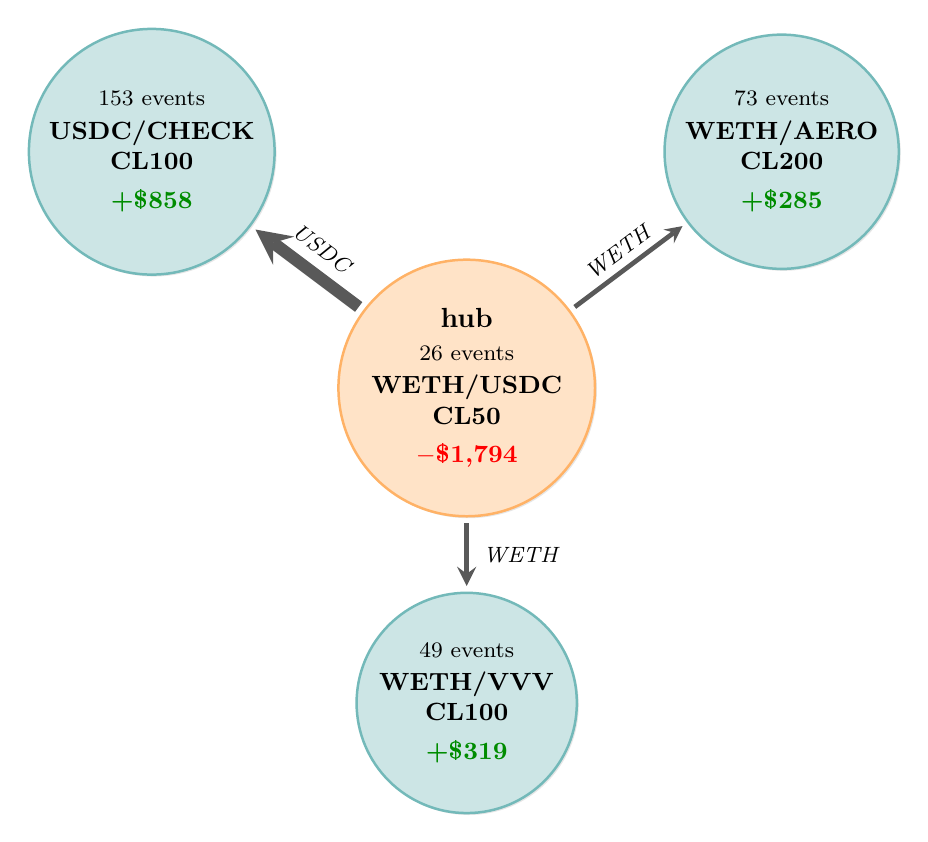
\begin{tikzpicture}[
  >=stealth,
  font=\small,
  hub/.style       = {circle, draw=orange!60, line width=0.9pt,
                      fill=orange!22, minimum size=3.1cm, align=center, inner sep=1pt,
                      drop shadow={shadow xshift=0.7pt, shadow yshift=-0.7pt, opacity=0.2}},
  spoke/.style     = {circle, draw=teal!55, line width=0.9pt,
                      fill=teal!20,   minimum size=2.7cm, align=center, inner sep=1pt,
                      drop shadow={shadow xshift=0.7pt, shadow yshift=-0.7pt, opacity=0.2}},
  flow/.style      = {->, draw=black!65, shorten >=2pt, shorten <=2pt},
  tok/.style       = {font=\footnotesize\itshape,
                      inner xsep=2pt, inner ysep=1pt},
]
% Hub at centre: HUB, events, position name, dollar amount
\node[hub] (hub) at (0,0) {%
  {\normalsize\textbf{\textsc{hub}}}\\[1pt]
  {\footnotesize 26 events}\\[1pt]
  \textbf{WETH/USDC}\\
  \textbf{CL50}\\[3pt]
  \textbf{\textcolor{red}{$-$\$1{,}794}}};

% Spokes: events, position name, dollar amount
\node[spoke] (s1) at (-4.0, 3.0) {%
  {\footnotesize 153 events}\\[1pt]
  \textbf{USDC/CHECK}\\
  \textbf{CL100}\\[3pt]
  \textbf{\textcolor{green!55!black}{+\$858}}};
\node[spoke] (s2) at ( 4.0, 3.0) {%
  {\footnotesize 73 events}\\[1pt]
  \textbf{WETH/AERO}\\
  \textbf{CL200}\\[3pt]
  \textbf{\textcolor{green!55!black}{+\$285}}};
\node[spoke] (s3) at ( 0.0,-4.0) {%
  {\footnotesize 49 events}\\[1pt]
  \textbf{WETH/VVV}\\
  \textbf{CL100}\\[3pt]
  \textbf{\textcolor{green!55!black}{+\$319}}};

% Connector arrows; line width scales with absorption magnitude
% (USDC/CHECK +$858, WETH/VVV +$319, WETH/AERO +$285)
\draw[flow, line width=4.4pt] (hub) -- node[tok, sloped, above=3pt, midway] {USDC} (s1);
\draw[flow, line width=1.7pt] (hub) -- node[tok, sloped, above=2pt, midway] {WETH} (s2);
\draw[flow, line width=2.0pt] (hub) -- node[tok, right=3pt, midway] {WETH} (s3);
\end{tikzpicture}
\caption{Hub-spoke topology in Group~B (Phase~2). Arrow thickness scales with cumulative absorption, and italic labels indicate the connector token.}
\label{fig:hub-spoke}
\end{figure}

Major hub donations were followed by spoke absorptions within about two hours. This pattern is consistent with WETH residuals emitted by the hub being absorbed by WETH-paired spokes on subsequent rebalances.

Unlike single-pool positions, multi-pool positions do not converge to equal value. The hub remains larger because WETH/USDC CL50 has deeper TVL and therefore lower $V/L_p$ at the same capital level. Equation~\eqref{eq:multipool} implies equilibrium position sizes proportional to pool depth.

\subsection{Regime analysis}\label{sec:regime}

The 41.9-hour Phase~1 window can be divided into five market-state sub-periods (Appendix~\ref{app:empirical}, Table~\ref{tab:regime}). On average, volatile positions shed capital during stress and absorbed capital during the subsequent recovery. Flow direction is therefore regime-dependent rather than fixed by position, which is consistent with mismatch widening under stress.

\subsection{Stablecoin FX isolation}\label{sec:fx-isolation}

Five stablecoin FX pairs deployed on a Sunday, when markets were closed and $\sigma \approx 0$, provide a control setting that isolates $V/L_p$ from volatility (Appendix~\ref{app:empirical}, Table~\ref{tab:fx}). No swaps occurred in any fiat rebalance (\texttt{amountIn = 0} in every rebalance call), so $D = \Delta R$ exactly.

ZARP ($V/L_p \approx 0.96$) donated a mean $27\%$ of its value per donation event. All five pairs were deployed with equal capital. ZARP shrank steadily, KRWQ and CADC grew, and the portfolio-level dust totals approximately netted out (sum $+\$250$). This cross-position pattern is consistent with $V/L_p$ as the dominant predictor when $\sigma$ is suppressed.

\subsection{The two-mechanism split}\label{sec:two-mechanism-split}

The closed-form $D/V$ was tested against 642 Phase~2 events. Of these, 611 ($95\%$) were same range and all had $\Delta R = 0$ as Theorem~\ref{thm:residual} predicts, yet showed non-zero dust flows ($\overline{|D|} = \$20$), which the Stage~2 redistribution mechanism explains. The remaining 31 ($5\%$) were range-change events and all had $\Delta R \neq 0$ ($\overline{|D|} = \$35$). Of the 28 with the current tick inside the old range, the formula predicts direction correctly in 19 ($70\%$). The gap between predicted $|\overline{\Delta R/V}| = 44\%$ and observed $|\overline{D/V}| = 2.7\%$ matches the ${\sim}94\%$ Stage~1 swap absorption rate (\S\ref{sec:two-mechanism}).

The same partition appears at production scale. In Phase~3, which contains 35{,}910 rebalance events, $78\%$ are same range and $22\%$ are range-changing. Cumulative dust flow is positive on the same range branch and negative on the range-change branch, matching the Stage~1/Stage~2 split. Range-change events generate geometric residuals and incur swap slippage; same range events redistribute accumulated dust.

The 95/5 split in the controlled Phase~2 dataset shifts to 78/22 in Phase~3 because the rebalancing engine was retuned to tighter ranges (mean width $\approx 181$ ticks in Phase~3 versus $\approx 528$ in Phase~2). This raised the exit rate from $0.5\%$ to $6.8\%$ and increased the share of range-change events. The sign pattern across branches is unchanged.

\subsection{Position extinction: the ZARP case study}\label{sec:zarp}

The USDC/ZARP CL10 position observed in Phase~2 provides an empirical trajectory consistent with Theorem~\ref{thm:extinction}, from deployment to extinction, with $S = 0$ on every event.

ZARP, a South African rand stablecoin, had no DEX swap route on Base. The Odos aggregator returned no path, so every rebalance reduced to a pure withdraw--mint sequence with no token ratio correction, giving $D = \Delta R$ exactly. The 14-event trajectory is reported in Appendix~\ref{app:empirical}, Table~\ref{tab:zarp}.

Total donated was \$1{,}528 and total absorbed \$587 across 4 events. Net flow was $-\$941$, or $99.8\%$ of initial capital.

The trajectory falls into three regimes. In events 1--4, $V/L_p > 0.95$ and the position donated on every rebalance. In events 5--8, $L_p$ fluctuated by $4\times$ and donation alternated with absorption. In events 9--14, $L_p$ increased $20\times$ between events 11 and 12, reducing $V/L_p$ to $0.001$. The final rebalance produced $\alpha = 0.99$.

\needspace{6\baselineskip}
\textbf{Extinction bound.} Theorem~\ref{thm:extinction}(iv) gives both a tighter bound based on $\bar\alpha$ and a looser bound based on $\alpha_{\min}$. With $\bar\alpha = 0.45$ across the 10 donation events,
\[
K^* = \left\lceil \frac{\ln(942/1.59)}{\ln(1/0.55)} \right\rceil = \lceil 10.7 \rceil = 11
\]
rebalances. Using $\alpha_{\min} = 0.16$ (Event~1, the smallest donation), the uniform a priori bound gives
\[
K_{\text{loose}}^* = \lceil 36.7 \rceil = 37
\]
rebalances.

The tighter bound predicts 11 donation rebalances, while 10 were observed. The remaining 4 events were absorption recoveries driven by exogenous changes in pool liquidity and therefore lie outside Theorem~\ref{thm:extinction}'s pure-decay regime. Accordingly, the bound is consistent with the observed trajectory.

\textbf{Recovery episodes.} The three largest absorption events (5, 8, and 12) each coincided with a marked increase in pool liquidity $L_p$. After each one, the position returned to donation on the next rebalance, consistent with the recovery condition in the irreversibility corollary.

\subsection{Directional asymmetry: production-scale check}\label{sec:directional-empirical}

Phases~1--2 above were controlled case studies: the $V/L_p$ sweep, the hub-spoke topology, and the ZARP lifecycle. Phase~3 is the production-scale dataset, with 35{,}910 events across 36 positions deployed in five independent portfolios. Each portfolio runs its own depositor-keyed dust pool, with its own connector-token structure and position composition, so the right unit of analysis is the portfolio rather than the pooled stream. Phase~3 therefore provides five independent replications of Theorem~\ref{thm:directional}.

Theorems~\ref{thm:directional} and~\ref{thm:exit} apply when the stablecoin sits at $T_1$. V3 assigns $T_0$ and $T_1$ by token address, lowest first, so the same stablecoin can land at $T_0$ in one pair and at $T_1$ in another. WETH/USDC places WETH at $T_0$ (theorem domain), while USDC/cbBTC places USDC at $T_0$ (reversed ordering). Non-USD fiat-pegged tokens (EURC, ZARP, VCHF, CADC, KRWQ) are volatile in USD terms, so pairs combining them with USDC, USDT, or DAI also fall inside the theorem domain. The reversed subset is a built-in negative control. Because the asymmetry is numéraire-induced, the inequality should attenuate or invert when V3 token roles flip.

Within each portfolio, the test compares mean dust on rising rebalances to mean dust on falling rebalances, with direction set by $|\Delta_{\mathrm{norm}}| > 0.1$. Theorem~\ref{thm:directional} predicts $\bar V_r > \bar V_f$ in the theorem domain. All five portfolios produce $\bar V_r > \bar V_f$ (Table~\ref{tab:directional-phase3}). Under the null of no directional asymmetry, each portfolio is independently equally likely to give either ordering, so $5/5$ corresponds to a one-sided sign-test $p = 1/32 \approx 0.031$.

\begin{table}[H]
\centering
\caption{Per-portfolio directional asymmetry.}
\label{tab:directional-phase3}
\begin{tabular}{@{}lrrrrrrrr@{}}
\toprule
 & & & & & & & \multicolumn{2}{c}{95\% CI} \\
\cmidrule(lr){8-9}
Portfolio & Events & $N_r$ & $N_f$ & $\bar V_r$ & $\bar V_f$ & Diff & Lo & Hi \\
\midrule
P1 & 21{,}810 & 5{,}413 & 2{,}622 & $+$\$104 & $+$\$1   & $+$\$102 & $-$\$4  & $+$\$263 \\
P2 & 7{,}066  & 935     & 457     & $+$\$5   & $+$\$1   & $+$\$3   & $-$\$28 & $+$\$38  \\
P3 & 3{,}391  & 793     & 214     & $+$\$20  & $-$\$36  & $+$\$56  & $-$\$31 & $+$\$153 \\
P4 & 2{,}163  & 496     & 189     & $+$\$7   & $-$\$18  & $+$\$25  & $+$\$5  & $+$\$46  \\
P5 & 1{,}479  & 579     & 134     & $+$\$3   & $-$\$13  & $+$\$16  & $+$\$4  & $+$\$33  \\
\bottomrule
\end{tabular}
\end{table}

Per-portfolio confidence intervals are wide. Per-event dust flow is heavy-tailed, with a few large rebalances dominating the means, so the 5{,}000-iteration bootstrap on the mean difference produces 95\% intervals that often span zero. The sign test is the appropriate summary because it is invariant to magnitude. The pooled production-scale figure, a $5\times$ rising/falling magnitude ratio across 27{,}022 directional events, conflates the five siphon systems and dilutes the per-portfolio signal.

The reversed-ordering negative control behaves as Theorem~\ref{thm:directional} predicts. The median per-portfolio (rising $-$ falling) drops from $+\$25$ in the theorem domain to about $+\$1$ in the reversed subset, attenuating as V3 token roles flip. The exit case in \S\ref{sec:exit-empirical} shows a sharper sign flip on the same control.

One caveat remains. The Phase~3 signal is the net dust flow $D = \Delta R - S$, with the residual $\Delta R$ itself unobserved, so the directional interpretation assumes the swap absorption fraction $S/\Delta R$ is approximately symmetric across directions; Phase~3's design does not test that assumption. Theorems~\ref{thm:directional} and~\ref{thm:exit} concern position value $V$; by Theorem~\ref{thm:residual}, $|\Delta R|/V$ depends only on range geometry and current price, so $|\Delta R|$ inherits both asymmetries.

\subsection{Exit asymmetry: production-scale check}\label{sec:exit-empirical}

Phase~3 contains 2{,}428 exit events, rebalances at which the current tick crossed a position boundary. The same per-portfolio framing applies, with each portfolio an independent replication of Theorem~\ref{thm:exit} and the V3 ordering rule of \S\ref{sec:directional-empirical} determining which exits fall inside the theorem domain.

Within each portfolio, the test compares mean dust on above-range exits to mean dust on below-range exits. Theorem~\ref{thm:exit} predicts $\bar V_a > \bar V_b$, that an above-range exit retains more USD value than a below-range exit. Four of five portfolios produce $\bar V_a > \bar V_b$ in their theorem domain (Table~\ref{tab:exit-phase3}). The fifth (P5) has only 14 exits combined and is underpowered; restricting to portfolios with $N_b \geq 20$ gives $4/4$ in the predicted direction, sign-test $p = 1/16 \approx 0.063$. Per-portfolio confidence intervals are again wide because exits are a smaller share of events than directional rebalances.

\begin{table}[H]
\centering
\caption{Per-portfolio exit asymmetry.}
\label{tab:exit-phase3}
\begin{tabular}{@{}lrrrrrrrr@{}}
\toprule
 & & & & & & & \multicolumn{2}{c}{95\% CI} \\
\cmidrule(lr){8-9}
Portfolio & Events & $N_a$ & $N_b$ & $\bar V_a$ & $\bar V_b$ & Diff & Lo & Hi \\
\midrule
P1 & 21{,}810 & 406 & 285 & $-$\$37  & $-$\$99  & $+$\$62  & $-$\$193 & $+$\$335 \\
P2 & 7{,}066  & 93  & 87  & $-$\$31  & $-$\$66  & $+$\$35  & $-$\$92  & $+$\$202 \\
P3 & 3{,}391  & 52  & 26  & $-$\$36  & $-$\$295 & $+$\$259 & $-$\$200 & $+$\$874 \\
P4 & 2{,}163  & 55  & 23  & $-$\$16  & $-$\$78  & $+$\$63  & $-$\$35  & $+$\$158 \\
P5 & 1{,}479  & 9   & 5   & $-$\$13  & $-$\$5   & $-$\$8   & $-$\$37  & $+$\$14  \\
\bottomrule
\end{tabular}
\end{table}

\noindent\textbf{Reversed-ordering negative control.} On reversed ordering pairs, Theorem~\ref{thm:exit} predicts a sign flip in the exit inequality, where the directional case in \S\ref{sec:directional-empirical} predicts only attenuation. P1 is the only portfolio with enough reversed ordering exits ($N_b = 22$) for a direct test. On its reversed subset, $\bar V_b$ turns from a loss to a gain and the inequality flips as predicted (Table~\ref{tab:exit-control}).

\begin{table}[H]
\centering
\caption{P1 reversed-ordering negative control.}
\label{tab:exit-control}
\begin{tabular}{@{}lrrrr@{}}
\toprule
Regime & $N_a$ & $N_b$ & $\bar V_a$ & $\bar V_b$ \\
\midrule
Theorem domain ($T_0$ USD-volatile) & 406 & 285 & $-$\$37  & $-$\$99 \\
Reversed ordering ($T_0$ USD-stable) & 41  & 22  & $-$\$146 & $+$\$42 \\
\bottomrule
\end{tabular}
\end{table}

With $T_0$ USD-stable, an above-range exit holds only $T_1$, the volatile token, at a depressed price; a below-range exit holds only $T_0$, the stablecoin, at full USD value. The roles of $V_{\text{above}}$ and $V_{\text{below}}$ from Theorem~\ref{thm:exit} are swapped, and the empirical inequality reverses with them.

\section{Computational verification}\label{sec:foundry}

All six theorems are computationally verified against unmodified Uniswap V3 contracts on Base mainnet through a 16-test Foundry suite. The canonical example, Test~1, mints a 1 WETH $+$ 2{,}500 USDC position across $\pm 500$ ticks around tick 73{,}135, displaces the price by $+200$ ticks, and rebalances into a $\pm 1{,}000$-tick range, returning 2{,}061 USDC to the depositor balance as the geometric residual. The control test (same setup, re-mint into the identical range) returns 29~wei ($<\!10^{-6}$ USD), the analytical zero up to integer-arithmetic floor.

The suite covers Theorems~\ref{thm:residual} and~\ref{thm:extinction} with mock-pool tests and four live fork tests against the Aerodrome Slipstream \texttt{NonfungiblePositionManager}. It covers Theorems~\ref{thm:monotonicity}--\ref{thm:exit} with mock-pool tests using exact V3 \texttt{TickMath} constants, together with two further live fork tests on the Slipstream WETH/USDC pool for the directional and exit asymmetries, bringing the fork-test total to six.

All six fork tests are pinned to Base block \texttt{43{,}175{,}000} (2026-03-10 10:42 UTC), inside the paper's Phase~2 data window, so both the qualitative claims and the captured numerical residuals are reproducible against an archive RPC. Test descriptions, assertion details, and reproduction commands are in Appendix~\ref{app:foundry-detailed}.

\section{Discussion}\label{sec:discussion}

The six theorems above characterise the geometric residual through the V3 amount equations, and the empirical results trace the same mechanism in both case studies and production-scale directional patterns. The rest of this section addresses three related issues: the architectural precondition behind the mechanism, empirical edge cases at the framework's boundaries, and the role of unit-of-account choice in the USD-denominated directional asymmetry.

\subsection{The architectural precondition}\label{sec:precondition}

The geometric residual arises on any CL rebalance that changes the required token ratio at the current price, and in that sense it has existed since Uniswap V3 launched in May 2021. In vault-per-pool architectures, it remains trapped within the position that produced it and usually appears only as a small capital-efficiency loss, hard to distinguish from slippage in standard PnL tracking. Depositor-level shared balances change that. By allowing residuals from one pool to be consumed by positions in another, they make the same residual visible as inter-position flow.

Theorem~\ref{thm:residual} applies to all Uniswap V3-style concentrated liquidity implementations. Cross-position flow further requires shared token balances across positions in different pools. When that condition holds, the Connector Rule (\S\ref{sec:connector}) can operate. Depositor-level multi-pool accounting is still uncommon in production CL management, but it is not unique to the PMV6--PMV9 family studied here; any protocol that adopts it becomes exposed to the same mechanism.

The fork test in \S\ref{sec:foundry-fork} checks this precondition directly. On a stock NFPM, which does not maintain shared depositor balances, no cross-position absorption occurs. A concurrent SSRN preprint\cite{secondoperator2026} formalises a graph-theoretic condition for cross-pool circulation (token degree $\geq 2$ in the portfolio graph) on a port of the Position Manager to Uniswap V3, and derives a directional-convexity scaling for symmetric sqrt-price displacements. That work does not address quantitative magnitudes, so the empirical ratios reported in \S\ref{sec:results} remain specific to the present single-operator dataset.

\subsection{Boundary cases}\label{sec:boundary}

\textbf{Same-pool oscillation.} Two EURC/USDC CL1 positions in Phase~1 showed oscillating flows, with consecutive events reversing sign $62\%$ of the time. This produced dissipation without meaningful cross-pool reallocation.

\textbf{Isolated tokens.} In Phase~1, cbETH/cbBTC donated $-\$2{,}413.49$, but no other position held cbETH, so the residual accumulated as unusable contract dust. Cross-position siphon flow therefore requires each portfolio token to appear in at least two positions.

\textbf{Fat tails.} Two of 23 FLOCK rebalances accounted for $96\%$ of its lifetime donation, showing that per-event dust flows are heavy-tailed.

\subsection{Direction, magnitude, and unit of account}\label{sec:direction-discussion}

The siphon moves tokens between positions according to geometric ratios. Valued in USD, the flows also reflect the price exposure of the moved tokens, so Theorems~\ref{thm:directional} and~\ref{thm:exit} add a USD-denominated bias to a mechanism that is itself directionally blind. The reversed-ordering negative control in \S\S\ref{sec:directional-empirical}--\ref{sec:exit-empirical} empirically confirms the numéraire-induced character of the asymmetry: when V3 token roles flip, the inequalities attenuate and the exit case sign-flips.

USD-denominated dust performance therefore mixes signal and artefact. The signal is the mechanism-level flow determined by geometry; the artefact is the direction introduced by the chosen num\'eraire. Distinguishing the two requires num\'eraire-invariant accounting or explicit segmentation by pool address ordering, the latter applied to the production-scale data in \S\S\ref{sec:directional-empirical}--\ref{sec:exit-empirical}. Neither is standard in current LP performance reporting.

Redeployment carries the same asymmetry. Either terminal exit can only be reopened in range by swapping into the missing token. Above-exits hold the full stablecoin balance, while below-exits hold only the depreciated volatile token. By Corollary~\ref{cor:exit-ratio}, redeployable capital at a below-exit displacement $d$ is a fraction $P'/\sqrt{P_a P_b}$ of the above-exit case and vanishes as the price moves further past the lower boundary. Across consecutive below-exits without a recovery move, the gap compounds. The compounding gap is the operational signature of Theorem~\ref{thm:exit} in a depreciating market.

\subsection{Limitations}\label{sec:limitations}

All empirical data come from one operator's positions on Aerodrome (Base). Theorem~\ref{thm:residual} guarantees that the residual exists on all V3-style implementations, but the empirical patterns reported here (the per-portfolio replications, the controlled-phase $95/5$ two-mechanism split, and the case-study magnitudes) are specific to this dataset and may differ under other protocols, fee structures, rebalancing engines, or pair compositions.

The two observation windows, 7 days and 12 days respectively, do not span a full market cycle. The adaptive rebalancing engine also creates a circular dependence between volatility, range width, and dust flow. No counterfactual run with per-position dust accounting was available.

Theorem~\ref{thm:extinction} is proved only for $S = 0$. The intermediate case $0 < S_{\text{eff}} < 1$, where $S_{\text{eff}}$ is the fraction of $\Delta R$ recovered by the swap, lies between the convergence regime of Theorem~\ref{thm:convergence} and the extinction regime of Theorem~\ref{thm:extinction}, but that boundary has not yet been characterised. Theorem~\ref{thm:convergence} and Corollary~\ref{cor:convergence-rate} also bound the inter-position convergence rate at $c$ only under value-preserving swap routing; extending the result to include slippage-induced losses is left for future work.

Theorems~\ref{thm:directional} and~\ref{thm:exit} are proved in token1 units. Measured in token0 units, the inequalities reverse, so the asymmetry is a consequence of the chosen unit of account. The USD interpretation holds when token1 is USDC, USDT, or DAI, or when token1's USD price is approximately stable over the rebalance interval.

\subsection{Future work}\label{sec:future}

A first priority is to quantify the net cost or benefit of the siphon relative to vault-per-pool (ALM) and static LP strategies through controlled comparisons over longer horizons. Preliminary evidence from 33 post-flip events is consistent with a correlation between ve(3,3) emission rates and siphon role assignment, but separating emission effects from concurrent market-regime shifts will require observation across multiple epoch cycles.

A second open question is strategic manipulation. An attacker able to coordinate rebalance timing across multiple positions may be able to extract value from the siphon, but the feasibility, cost, and practical constraints of such an attack remain unknown.

On the modelling side, the closed-form formula predicts the signed residual $\Delta R$ before swap absorption, whereas precise net prediction of the observed $D = \Delta R - S$ requires an explicit model of the swap absorption fraction. In the present data, that fraction is about $94\%$. A unified growth equation,
\[
\frac{\dot V}{V} = g(V/L_p, \sigma, S_{\text{eff}}),
\]
that continuously interpolates between Theorems~\ref{thm:convergence} and~\ref{thm:extinction} would help characterise the transition boundary.

An immediate empirical next step is replication on a second operator's portfolios with independent V3 ordering composition, to confirm that the per-portfolio directional and exit asymmetries generalise beyond the present single-operator setting.

\section{Conclusion}\label{sec:conclusion}

When concentrated liquidity positions share a depositor-level token balance, autonomous rebalancing can generate systematic inter-position capital transfers implied by the geometry of the V3 amount equations. Six theorems characterise the residual, its long-run behaviour, and its directional and exit asymmetries on volatile/stablecoin pairs in V3 ordering. The cross-pool \emph{Connector Rule} is supported empirically but remains conjectural. A Foundry test suite verifies the theorem statements against unmodified V3 contracts.

The single-operator dataset of 1{,}380 events supports the existence claim and includes a complete USDC/ZARP extinction lifecycle. The position falls from \$942 to \$1.59 over 14 zero-swap rebalances, against a tighter bound of 11 at the average residual fraction. The 35{,}910-event production-scale dataset, across five independent portfolios, replicates the directional asymmetry in every portfolio, the exit asymmetry in four of five, and exhibits the predicted sign flip in the largest portfolio's reversed-ordering negative control.

The mechanism follows directly from the V3 amount equations once depositor-level shared balances are present. Any protocol that adopts that architecture is subject to it.

\backmatternotes

\section*{Acknowledgements}

The author thanks members of the DeFinancier Social Club for helpful discussion, testing feedback, and observations, and his fianc\'ee Ernesta, who looked after their young child and provided patient support during the work that produced this paper.

\section*{Author contributions}

K.\,R.\,R.\ conceived the study, derived the theorems, conducted the empirical analysis, implemented and ran the Foundry verification suite, and wrote the manuscript.

\section*{Conflict of interest}

The author operates the off-chain concentrated liquidity rebalancing system from which the empirical data in this paper were collected. All rebalance events analysed here are on-chain transactions on Aerodrome (Base). The author declares no other competing financial interests. No external funding supported this research.

\section*{Data and code availability}

The Foundry verification suite is publicly available on GitHub at \url{https://github.com/g4nc0r/the-geometric-siphon}, with an immutable archival snapshot on Zenodo at \url{https://doi.org/10.5281/zenodo.19905208}. A clean checkout reproduces every theorem verification described in \S\ref{sec:foundry}. The diffusion-event logs supporting the empirical analyses in \S\S\ref{sec:decomposition}--\ref{sec:exit-empirical}, together with a Python reproduction harness that regenerates the empirical tables and the V3 ordering classification used for the segmented Phase~3 analysis, are deposited on Zenodo at \url{https://doi.org/10.5281/zenodo.19904832}.

\bibliographystyle{manuscript}
\bibliography{references}

\appendix
\setcounter{section}{0}
\renewcommand{\thesection}{\Alph{section}}
\setcounter{secnumdepth}{2}

\titleformat{\subsection}{\fontshape{it}\selectfont\bfseries}{\thesubsection.}{0.5em}{}
\titlespacing*{\subsection}{0pt}{10pt}{4pt}

\titleformat{\subsubsection}[runin]{\fontshape{it}\selectfont\bfseries}{}{0pt}{}[.]
\titlespacing*{\subsubsection}{0pt}{6pt}{0.5em}

\section{Contract architecture}\label{app:contract}

\AtBeginEnvironment{verbatim}{\small}

\begin{verbatim}
// Dust balance keyed by depositor and token, no pool dimension
mapping(address => mapping(address => uint256)) public dustBalance;

// Atomic rebalance: withdraw -> optional swap -> mint -> stake
function rebalanceCL(
    address pool, uint256 tokenId,
    int24 newTickLower, int24 newTickUpper,
    uint256 amount0Min, uint256 amount1Min,
    uint256 deadline,
    SwapParams swapParams
) external returns (uint256 newTokenId);
\end{verbatim}

The \texttt{dustBalance[depositor][token]} keying makes leftover tokens from any pool's rebalance accessible to any subsequent mint under the same depositor; a vault-per-pool architecture instead uses \texttt{dustBalance[pool][token]} (or equivalent), isolating residuals per pair.

\section{Detailed derivations}\label{app:dr-derivation}

\setlength{\abovedisplayskip}{10pt plus 2pt minus 2pt}
\setlength{\belowdisplayskip}{10pt plus 2pt minus 2pt}
\setlength{\abovedisplayshortskip}{8pt plus 1pt minus 1pt}
\setlength{\belowdisplayshortskip}{8pt plus 1pt minus 1pt}

\subsection{Notation and setup}

Table~\ref{tab:notation} summarises the symbols used throughout the paper.

\begin{table}[H]
\centering
\caption{Notation used throughout the paper.}
\label{tab:notation}
\footnotesize
\renewcommand{\arraystretch}{1.05}
\begin{tabular}{@{}cL{10cm}@{}}
\toprule
Symbol & Meaning \\
\midrule
$s, s_a, s_b$ & current sqrt price; lower and upper sqrt-price bounds of the range \\
$s_a', s_b'$ & lower and upper sqrt-price bounds of the new range after a rebalance \\
$w = s_b - s_a$ & range width in sqrt-price space \\
$\delta$ & displacement of $s$ from the range midpoint \\
$\hat{\delta} = \delta/(w/2)$ & normalised displacement ($0$ at centre, $\pm 1$ at edge) \\
$L$ & position liquidity \\
$L_p$ & total in-range liquidity of the containing pool \\
$x, y$ & token0 and token1 amounts \\
$x_w, y_w$ & withdrawn token0 and token1 amounts on a rebalance \\
$T_0, T_1$ & token0 and token1; in Thms~\ref{thm:directional}--\ref{thm:exit}, $T_0$ is the volatile asset by convention and $T_1$ the stablecoin \\
$V$ & position value in token1 units (USD when $T_1$ is a stablecoin) \\
$\phi(s, s_a, s_b)$ & per-unit-liquidity value, $V = L\,\phi$ \\
$R(s, s_a, s_b)$ & token ratio $x/y$ required by range $[s_a, s_b]$ at price $s$ \\
$\Delta R$ & signed geometric residual value of an isolated rebalance \\
$S$ & swap slippage absorbed by the internal rebalance swap \\
$D = \Delta R - S$ & observed net dust flow per event \\
$D_{\text{pool}}$ & accumulated contract dust available for absorption \\
$\alpha, \bar\alpha, \alpha_{\min}$ & per-event residual fraction in zero-swap rebalances; running mean; minimum \\
$K^*$ & bound on the number of zero-swap rebalances to extinction \\
$\sigma$ & realised volatility over the rolling window used by the rebalancing engine \\
\bottomrule
\end{tabular}
\end{table}

The derivations below build on equations~\eqref{eq:amounts}--\eqref{eq:mint} from \S\ref{sec:residual}; throughout, $\phi(s, s_a, s_b)$ denotes the per-unit-liquidity value factor defined there.

\subsection{Theorem~\ref{thm:residual}: vanishing condition}

We restate the key claim for convenience before giving the substitution argument for the ratio-preserving branch.

\noindent\emph{Geometric residual.} For a concentrated liquidity rebalance from range $[s_a, s_b]$ to $[s_a', s_b']$ at current sqrt price $s$, with $s$ contained in both ranges, consider the isolated case in which no shared balance tokens contribute to the mint. Let $\Delta R = V_{\text{new}} - V_{\text{old}}$ denote the signed residual value of the rebalance. Then
\[
\frac{\Delta R}{V} = 0 \;\iff\; R(s, s_a, s_b) = R(s, s_a', s_b').
\]
Equivalently, the rebalance has zero residual value if and only if the old and new ranges require the same token ratio at the current price.

\subsubsection*{Direct substitution for the $(\Leftarrow)$ direction}

Suppose $R_{\text{old}} = R_{\text{new}}$. Then the withdrawn amounts $(x_w, y_w)$ already satisfy the ratio required by the new range, so both tokens redeploy in full and
\[
L_{\text{new}} = L\,\frac{s - s_a}{s - s_a'}.
\]
Substituting the ratio-preserving condition into the value factor gives
\[
\phi(s, s_a', s_b') = \frac{s - s_a'}{s - s_a}\,\phi(s, s_a, s_b).
\]
Hence
\[
V_{\text{new}}
= L_{\text{new}}\,\phi(s, s_a', s_b')
= L\,\frac{s - s_a}{s - s_a'} \cdot \frac{s - s_a'}{s - s_a}\,\phi(s, s_a, s_b)
= L\,\phi(s, s_a, s_b)
= V_{\text{old}},
\]
so $\Delta R/V = 0$.

\subsubsection*{Ratio-preserving locus}

At fixed $s$, the set of ranges satisfying
\[
R(s, s_a', s_b') = R_{\text{old}}
\]
is the zero set of
\[
(1/s - 1/s_b')(s - s_a) - (1/s - 1/s_b)(s - s_a') = 0.
\]
This is one equation in two unknowns and therefore generically defines a one-dimensional curve in the $(s_a', s_b')$ plane. The original range $(s_a, s_b)$ lies on that curve, but does not exhaust it.

\subsection{Theorem~\ref{thm:convergence} and Corollary~\ref{cor:convergence-rate}}

The convergence result is driven by size-proportional donation and size-inverse absorption.

\subsubsection*{Growth equation}

With per-position rebalance probability $\pi = 1/N$,
\begin{equation}\label{eq:growth-app}
\mathbb{E}\!\left[\frac{\dot{V}_i}{V_i}\right]
=
\frac{\pi D_{\text{pool}}}{V_i} - c.
\end{equation}

Across pools with total liquidities $L_{p,k}$, the same argument gives
\begin{equation}\label{eq:multipool-app}
\frac{V_i}{L_{p,k(i)}}
=
\frac{V_j}{L_{p,k(j)}}
\qquad \forall\, i,j.
\end{equation}

\subsubsection*{Spectral proof of Corollary~\ref{cor:convergence-rate}}

Let $\eta_i = V_i - \bar V$, where $\bar V$ is the equilibrium value, and let $\eta = (\eta_1, \ldots, \eta_N)^T$. Conservation of total value implies
\[
\sum_j \eta_j(t) = -\bigl(D_{\text{pool}}(t) - D_{\text{pool}}^*\bigr),
\qquad
D_{\text{pool}}^* = \frac{c\bar V}{\pi}.
\]
Linearising at the fixed point gives
\[
\dot\eta_i = -c\,\eta_i - \pi \sum_j \eta_j,
\]
or
\[
\dot\eta = -M\eta,
\qquad
M = cI + \pi\,\mathbf{1}\mathbf{1}^T.
\]
The matrix $M$ has eigenvalue $c + N\pi$ in the $\mathbf{1}$ direction and eigenvalue $c$ on the orthogonal $(N-1)$-dimensional subspace. Thus common-mode perturbations decay at rate $c + N\pi$, while inter-position differences decay at rate $c$.

\subsection{Theorem~\ref{thm:extinction}: product bound and extinction time}

The bound in Theorem~\ref{thm:extinction} follows from repeated application of the one-step leak and an AM--GM inequality.

\subsubsection*{AM--GM derivation}

Iterating the one-step update gives
\[
V_K = V_0 \prod_{k=1}^{K} (1 - \alpha_k),
\qquad 0 < \alpha_k < 1.
\]
Applying AM--GM to the factors $\{1-\alpha_k\}_{k=1}^K$ yields
\[
\Bigl(\prod_{k=1}^K (1 - \alpha_k)\Bigr)^{1/K}
\leq
\frac{1}{K}\sum_{k=1}^K (1 - \alpha_k)
=
1 - \bar\alpha_K,
\]
where
\[
\bar\alpha_K = \frac{1}{K}\sum_{k=1}^K \alpha_k.
\]
Hence
\[
V_K \leq V_0(1 - \bar\alpha_K)^K.
\]
Since $1 - \alpha_k \leq 1 - \alpha_{\min}$ for all $k$, we also have
\[
V_K \leq V_0(1 - \alpha_{\min})^K.
\]
If $\bar\alpha$ denotes a fixed mean residual fraction, the condition
\[
V_0(1 - \bar\alpha)^K \leq \varepsilon
\]
is equivalent to
\[
K \geq \frac{\ln(V_0/\varepsilon)}{\ln(1/(1-\bar\alpha))},
\]
which gives the stated ceiling bound.

\subsection{Theorem~\ref{thm:monotonicity}: derivative simplification}

For the equal-width recentred rebalance,
\begin{equation}\label{eq:dr-closed-form-app}
\Delta R(\delta) = L(s - s_a) - L\!\left(\frac{1/s - 1/s_b}{1/s - 1/(s + w/2)}\right)(w/2).
\end{equation}
With $s = \bar s + \delta$, $s_a = \bar s - w/2$, and $s_b = \bar s + w/2$, use
\[
1/s - 1/s_b = \frac{s_b - s}{s s_b},
\qquad
1/s - 1/(s + w/2) = \frac{w/2}{s(s + w/2)}.
\]
The factors of $s$ cancel, giving
\begin{equation}\label{eq:g-simplified}
\Delta R(\delta)
=
L\,(w/2 + \delta)
-
L\,\frac{(w/2 - \delta)(\bar s + \delta + w/2)}{\bar s + w/2}.
\end{equation}
Differentiating yields
\[
\frac{d\,\Delta R}{d\delta}
=
L\,\frac{2\bar s + 2\delta + w/2}{\bar s + w/2},
\]
which is strictly positive on \((0,w/2]\), establishing strict monotonicity on the upward branch. The same calculation with $\delta \to -\delta$ shows the downward branch is also strictly monotone in $|\delta|$, with boundary magnitude $|\Delta R(-w/2)| = L \cdot w \cdot \bar{s}/s_b < L \cdot w$ (Theorem~\ref{thm:directional}).

\subsection{Theorems~\ref{thm:directional} and~\ref{thm:exit}: directional identities}

\subsubsection*{Directional identity}

The USD-value gap between symmetric up- and down-moves is
\begin{equation}\label{eq:directional-identity-app}
V(s + \delta) - V(s - \delta)
= 4L\delta\left(1 - \frac{s}{s_b}\right).
\end{equation}
Since $s < s_b$ in the interior of the range, the factor in parentheses is strictly positive.

\subsubsection*{Price-space scaling}

\begin{corollary}[Leading-order price-space scaling]\label{cor:directional-scaling}
For a position with $s$ in the interior of $[s_a, s_b]$, a symmetric price-space displacement of magnitude $\Delta P$ around the current price $P_0 = s^2$ produces, to leading order in $\Delta P/P_0$, a USD-value gap
\[
V(P_0 + \Delta P) - V(P_0 - \Delta P)
=
\frac{2L\,\Delta P}{\sqrt{P_0}}
\left(1 - \sqrt{\frac{P_0}{P_b}}\right)
+
O\!\left((\Delta P/P_0)^2\right),
\]
where $P_b = s_b^2$ is the upper-range price.
\end{corollary}

This follows by substituting
\[
\delta = \frac{\Delta P}{2s} + O\!\left((\Delta P/P_0)^2\right)
\]
into~\eqref{eq:directional-identity-app}, with $s = \sqrt{P_0}$.

\subsubsection*{Below-exit value and exit ratio}

At a below-range exit,
\begin{equation}\label{eq:vbelow-app}
V_{\text{below}}(d) = L\left(\frac{1}{s_a} - \frac{1}{s_b}\right)(s_a - d)^2.
\end{equation}
Therefore
\[
\frac{V_{\text{below}}(d)}{V_{\text{above}}}
=
\frac{(s_a - d)^2}{s_a s_b}
=
\frac{P'}{\sqrt{P_a P_b}},
\]
with $P' = (s_a-d)^2$, $P_a = s_a^2$, and $P_b = s_b^2$.

\section{Foundry test suite reproduction}\label{app:foundry}

\AtBeginEnvironment{verbatim}{\small}

The full verification suite comprises 16 tests across 5 contracts, with the test--theorem mapping given in \S\ref{sec:foundry}. Reproducing the suite requires Foundry \texttt{forge} and, for the fork-based tests, any working Base RPC endpoint.

The mock-pool tests run locally without network access:

\begin{verbatim}
forge test -vv --no-match-contract "(GeometricResidualProof|DirectionalExitForkProof)$"
\end{verbatim}

The full suite, including the 6 live fork tests, runs with:

\begin{verbatim}
RPC_BASE_ALCHEMY=https://mainnet.base.org forge test -vv
\end{verbatim}

Recorded \texttt{forge test -vv} output corresponding to the subsections of \S\ref{sec:foundry} is provided in \texttt{foundry/PROOF\_OUTPUT.md} and serves as the deterministic regression target for the mock-pool tests.

\section{Foundry test descriptions}\label{app:foundry-detailed}

\AtBeginEnvironment{tabular}{\footnotesize}
\renewcommand{\arraystretch}{1.0}
\setlength{\tabcolsep}{5pt}

This appendix describes the 16 tests summarised in \S\ref{sec:foundry}. The mock-pool tests (Tests 1--10) use Solidity integer arithmetic, which can floor very small token0 values to zero at depressed prices and thereby mask strict monotonicity in some directional and exit cases (Tests 5, 9, 10). The fork tests on unmodified Slipstream contracts do not exhibit this display floor.

\subsection{Test 1: Range change creates residual}\label{sec:foundry-mock-residual}

Setup, observed values, and assertion are reported in \S\ref{sec:foundry}; the 2{,}061 USDC residual matched expectation.

\subsection{Test 2: Same range = zero residual (control)}\label{sec:foundry-mock-control}

Same setup and price movement as Test~1, but re-minting into the identical range. The residual was 29 wei.

\subsection{Test 3: Linear scaling with position size}\label{sec:foundry-mock-scaling}

\begin{table}[H]
\centering
\caption{Mock-pool position-size scaling.}
\label{tab:foundry-scaling}
\begin{tabular}{@{}lrl@{}}
\toprule
Position size & Residual & Ratio \\
\midrule
0.5 WETH & 1{,}030 & $1.0\times$ \\
2.0 WETH & 4{,}122 & $4.00\times$ \\
\bottomrule
\end{tabular}
\end{table}

\noindent A fourfold increase in position size produced a fourfold increase in the residual.

\subsection{Test 4: Single-sided exit with no swap (Theorem~\ref{thm:extinction}, part i)}\label{sec:foundry-mock-extinction}

A 1 WETH $+$ 2{,}500 USDC position over $[72800, 73000]$ was pushed $+200$ ticks above the upper bound. Withdrawal returned 0 WETH and 2{,}499{,}999{,}999 USDC. Re-minting into $[73000, 73400]$, which requires both tokens, produced zero liquidity, leaving a residual of $100\%$ of position value ($\alpha = 1.0$).

\subsection{Test 5: Residual scales with displacement (Theorem~\ref{thm:extinction}, part ii)}\label{sec:foundry-displacement}

Position deployed with $1{,}000$-tick range; price displaced past upper boundary:

\begin{table}[H]
\centering
\begin{tabular}{@{}lr@{}}
\toprule
Displacement & $\alpha$ \\
\midrule
100 ticks & $0\%$ \\
300 ticks & $37\%$ \\
600 ticks & $100\%$ \\
\bottomrule
\end{tabular}
\end{table}

\noindent The residual fraction rose strictly with displacement. The $\alpha = 0\%$ value at 100 ticks is the mock-pool integer-floor artefact noted above; on real V3 \texttt{TickMath} it is small but strictly positive.

\subsection{Test 6: Geometric decay over repeated rebalances (Theorem~\ref{thm:extinction}, part iii)}\label{sec:foundry-decay}

Five sequential rebalance cycles with 150-tick price drift and no swap:

\begin{table}[H]
\centering
\begin{tabular}{@{}rrr@{}}
\toprule
Cycle & Value (USD) & Decay factor \\
\midrule
0 & 4{,}999 & --- \\
1 & 3{,}823 & 0.76 \\
2 & 1{,}565 & 0.40 \\
3 & 1{,}197 & 0.76 \\
4 & 490     & 0.40 \\
5 & 374     & 0.76 \\
\bottomrule
\end{tabular}
\end{table}

\noindent Total decay was $92\%$ over five cycles. The alternating $0.76 / 0.40$ factors reflect the token ratio flip at each step; their two-step product $0.76 \times 0.40 = 0.30$ is the effective decay constant.

\subsection{Test 7: Deep out-of-range terminal event (Theorem~\ref{thm:extinction}, extreme case)}\label{sec:foundry-terminal}

Repeats the setup of Test~4 at an extreme 2{,}000-tick displacement above the upper bound. New liquidity was zero and the residual fraction was $\alpha = 100\%$, mirroring the ZARP terminal event in \S\ref{sec:zarp} (Event~14, $\alpha = 0.99$).

\subsection{Live fork verification (Theorems~\ref{thm:residual},~\ref{thm:extinction})}\label{sec:foundry-fork}

Four fork tests run against the live Aerodrome Slipstream WETH/USDC pool on Base mainnet, calling the unmodified \texttt{NonfungiblePositionManager} via \texttt{vm.createSelectFork}. They reproduce the range-change residual, the same range control, position-size scaling, and the architectural precondition (\S\ref{sec:precondition}). Fork residuals are about \$329 at the pinned block (Base \texttt{43{,}175{,}000}, mid-Phase~2), smaller than mock-pool residuals because the fork tests swap a fixed \$1{,}000 USDC and shift only 1--3 ticks; the qualitative claim is independent of magnitude.

The architectural-precondition test creates two positions in the same range, leaves a residual via the first, and confirms that the second position's liquidity does not increase on a same range rebalance. In a stock NFPM there is no shared dust balance, so no cross-position absorption occurs. Theorems~\ref{thm:directional} and~\ref{thm:exit} are verified on the same pool in fork tests pinned to the same block; results are in \S\S\ref{sec:foundry-fork-directional}--\ref{sec:foundry-fork-exit}.

\subsection{Test 8: Residual monotonicity (Theorem~\ref{thm:monotonicity})}\label{sec:foundry-monotonicity}

Five in-domain displacement levels were tested on a $1{,}000$-tick-wide position at price ${\sim}\$2{,}500$, so $|\delta| \leq w/2 = 500$ ticks. Dust rose strictly with displacement: \$1{,}822 at $+100$ ticks, \$3{,}663 at $+200$, \$5{,}522 at $+300$, \$7{,}400 at $+400$, and \$9{,}297 at the $+500$-tick range exit. The sequence gave zero violations of monotonicity within the theorem's domain.

\subsection{Test 9: Directional asymmetry (Theorem~\ref{thm:directional})}\label{sec:foundry-directional}

Five symmetric displacement levels were tested on a \$5{,}000 position. In the first four rows, both displaced prices remain strictly inside the range, which is the domain of Theorem~\ref{thm:directional}. In the fifth row ($\pm 450$ ticks), the down-move reaches the lower range boundary $s_a$. The up-move strictly exceeded the down-move at all five displacement levels (e.g.\ $V_{\text{up}} = \$5{,}522$ vs $V_{\text{down}} = \$3{,}663$ at $\pm 100$ ticks; $V_{\text{up}} = \$8{,}346$ vs $V_{\text{down}} = \$908$ at $\pm 400$ ticks), and the gap widened monotonically with displacement. In the $\pm 450$-tick row, the down-move displays as \$0 because of the mock-pool integer floor discussed in the appendix preamble; Test~11 verifies the same theorem on the live Slipstream WETH/USDC pool with that floor absent.

\subsection{Test 10: Exit asymmetry (Theorem~\ref{thm:exit})}\label{sec:foundry-exit}

Five symmetric exit distances past the range boundary were tested ($\pm 50$, $\pm 100$, $\pm 200$, $\pm 300$, $\pm 500$ ticks). The above-exit position retained its full \$9{,}297 stablecoin value at all five distances, while the below-exit displayed as \$0 under the integer floor. The swap fraction required to redeploy was 0~bps from the above-exit state and 9{,}999~bps from the below-exit state, at every distance. Both $V_{\text{above}} > V_{\text{below}}$ and the swap fraction gap therefore held throughout. Strict monotonicity in $d$ is masked here by the floor; Test~12 resolves $V_{\text{below}}$ to a strictly positive value on the live Slipstream pool.

\subsection{Test 11: Directional asymmetry on live Slipstream (Theorem~\ref{thm:directional})}\label{sec:foundry-fork-directional}

A $\pm 1{,}000$-tick position was minted on the live Slipstream WETH/USDC pool (WETH at $T_0$, USDC at $T_1$, matching the theorem ordering) and the price was displaced upward and downward from a common post-mint snapshot. $V_{\text{up}} > V_{\text{down}}$ held, resolving the inequality on real V3 \texttt{TickMath} without the mock-pool floor.

\subsection{Test 12: Exit asymmetry on live Slipstream (Theorem~\ref{thm:exit})}\label{sec:foundry-fork-exit}

A narrower position (one tick spacing either side of the current tick) was minted on the same pool and the price was pushed past each boundary in turn. The above-exit state held only USDC; the below-exit state held only WETH at a depressed price. $V_{\text{above}} > V_{\text{below}}$ held, with $V_{\text{below}}$ strictly positive on the live pool.

\section{Empirical detail tables}\label{app:empirical}

\begin{table}[H]
\centering
\caption{$V/L_p$ transfer function (Phase~2 cross-position scatter through 9~March, $N = 606$).}\label{tab:vl-buckets}
\begin{tabular}{@{}lrrl@{}}
\toprule
$V/L_p$ range & $N$ & Mean $D/V$ & Behaviour \\
\midrule
$< 0.01$       & 445 (73\%) & $+0.002$ & Near zero; position negligible relative to pool \\
$0.01$--$0.05$ & 98         & $+0.008$ & Mild absorption \\
$0.05$--$0.10$ & 29         & $+0.065$ & Peak absorption \\
$0.10$--$0.20$ & 20         & $-0.006$ & Crossover zone \\
$0.20$--$0.50$ & 9          & $-0.034$ & Consistent donation \\
$0.50$--$1.00$ & 5          & $-0.069$ & Strong donation; position dominates pool \\
\bottomrule
\end{tabular}
\end{table}

\begin{table}[H]
\centering
\caption{Cross-group token decomposition (395 transaction receipts across 10 pools and 5 depositor groups).}
\label{tab:cross-group}
\begin{tabular}{@{}llcrrr@{}}
\toprule
Pool & Group & Driver & Driver $r$ & Other $r$ & $N$ \\
\midrule
CLAWD/USDC       & A & CLAWD       & $-0.98$ & $-0.42$ & 62 \\
WETH/USDC        & A & WETH        & $-0.98$ & $-0.31$ & 38 \\
WETH/AERO        & A & AERO        & $-0.94$ & $-0.28$ & 31 \\
WETH/VVV         & B & WETH        & $-0.89$ & $-0.15$ & 47 \\
WETH/AERO        & B & WETH        & $-0.97$ & $-0.27$ & 73 \\
WETH/USDC        & B & USDC        & $-0.56$ & $-0.40$ & 25 \\
EURC/USDC        & C & USDC        & $-0.55$ & ---     & 9  \\
WETH/USDC        & D & USDC        & $-0.68$ & $-0.56$ & 17 \\
KellyClaude/USDC & E & KellyClaude & $-0.68$ & $-0.60$ & 20 \\
\bottomrule
\end{tabular}
\end{table}

\begin{table}[H]
\centering
\caption{Hub-spoke topology in Group~B, cumulative dust flows across 301 events.}\label{tab:hubspoke}
\begin{tabular}{@{}llrr@{}}
\toprule
Position & Role & Cumulative dust flow & Events \\
\midrule
WETH/USDC CL50 (hub) & Donor    & $-\$1{,}794$ & 26 \\
USDC/CHECK CL100     & Absorber & $+\$858$              & 153 \\
WETH/AERO CL200      & Absorber & $+\$285$              & 73 \\
WETH/VVV CL100       & Absorber & $+\$319$              & 49 \\
\bottomrule
\end{tabular}
\end{table}

\begin{table}[H]
\centering
\caption{Phase~1 regime partitioning by market state.}\label{tab:regime}
\begin{tabular}{@{}llrrl@{}}
\toprule
Phase & Period (UTC) & Events & Net \$ & Market character \\
\midrule
P1: Stress      & 03 Mar 17:49 -- 04 Mar 06:00 & 217 & $-\$196$ & ETH $\$2{,}215 \to \$1{,}984$ \\
P2: Recovery    & 04 Mar 06:00 -- 12:00         & 137 & $+\$960$ & Volatility subsides \\
P3: Rally       & 04 Mar 12:00 -- 20:45         & 170 & $-\$240$ & BTC $\to \$71.4$K \\
P4: Post-Rally  & 04 Mar 20:45 -- 05 Mar 04:34  & 147 & $-\$323$ & Consolidation \\
P5: Calm        & 05 Mar 04:34 -- 11:47         & 67  & $+\$86$  & Diverse portfolios stabilise \\
\bottomrule
\end{tabular}
\end{table}

\begin{table}[H]
\centering
\caption{Stablecoin-FX isolation, five positions deployed while markets were closed ($\sigma \approx 0$).}\label{tab:fx}
\begin{tabular}{@{}lrrrr@{}}
\toprule
Position & $V/L_p$ & $\sigma_{24h}$ & Cumulative dust flow & Swaps \\
\midrule
ZARP & 0.958 & 98.8 & $-\$601$ & 0 \\
VCHF & 0.034 & 1.4  & $+\$72$            & 0 \\
CADC & 0.003 & 5.0  & $+\$131$           & 0 \\
KRWQ & 0.025 & 1.5  & $+\$432$           & 0 \\
EURC & 0.001 & 0.1  & $+\$216$           & 0 \\
\bottomrule
\end{tabular}
\end{table}

\begin{table}[H]
\centering
\caption{USDC/ZARP CL10 extinction trajectory over 14 rebalance events.}
\label{tab:zarp}
\setlength{\tabcolsep}{4pt}
\renewcommand{\arraystretch}{0.9}
\begin{tabular}{@{}rllrrrrrr@{}}
\toprule
Event & Time (UTC) & Pre (\$) & Post (\$) & Dust $D$ & $V/L_p$ & $\alpha$ & $L_p$ \\
\midrule
1  & 07 Mar 17:05 & 942 & 791  & $-\$152$ & 0.958 & 0.16 & 135M \\
2  & 07 Mar 19:30 & 791 & 532  & $-\$259$ & 0.974 & 0.33 & 223M \\
3  & 08 Mar 05:02 & 532 & 338  & $-\$194$ & 0.992 & 0.36 & 693M \\
4  & 08 Mar 13:27 & 338 & 170  & $-\$168$ & 0.960 & 0.50 & 144M \\
5  & 08 Mar 22:31 & 170 & 342  & $+\$171$ & 0.790 & ---  & 352M \\
6  & 09 Mar 00:24 & 342 & 171  & $-\$171$ & 0.598 & 0.50 & 232M \\
7  & 09 Mar 04:37 & 170 & 51   & $-\$119$ & 0.448 & 0.70 & 93M \\
8  & 09 Mar 04:46 & 51  & 281  & $+\$229$ & 0.976 & ---  & 235M \\
9  & 09 Mar 10:18 & 280 & 235  & $-\$45$  & 0.971 & 0.16 & 197M \\
10 & 09 Mar 11:08 & 235 & 188  & $-\$47$  & 0.966 & 0.20 & 158M \\
11 & 09 Mar 13:47 & 187 & 77   & $-\$111$ & 0.917 & 0.59 & 68M \\
12 & 09 Mar 16:40 & 77  & 248  & $+\$172$ & 0.152 & ---  & 1{,}341M \\
13 & 09 Mar 21:28 & 249 & 264  & $+\$15$  & 0.159 & ---  & 1{,}353M \\
14 & 10 Mar 09:52 & 264 & 1.59 & $-\$262$ & 0.001 & 0.99 & 1{,}137M \\
\bottomrule
\end{tabular}
\end{table}

\thispagestyle{pagelast}

\end{document}
